% \chapter{Sensing Soft Robots' Shape with Cameras: An Investigation on Kinematics-Aware SLAM}
\chapter{Shape Sensing with Cameras: An Investigation on Kinematics-Aware SLAM}
\label{chp:srslam}

\begin{foreword}
    Before we can develop advanced soft robot controllers, we require access to state information. Specifically, we need to know the configuration of the soft robot, which, as introduced in Chapter~\ref{chp:background}, is for soft robots usually defined as the parametrized shape of the backbone.
    In this chapter, we demonstrate how we can augment in a plug-and-play fashion existing state-of-the-art \gls{SLAM} algorithms with kinematic knowledge to achieve shape sensing for soft robots.
\end{foreword}

\begin{abstract}
    % The nature of continuum soft robots calls for novel perception solutions, which can provide information on the robot's shape while not substantially modifying their bodies' softness. One way to achieve this goal is to develop innovative and completely deformable sensors. 
    One way to achieve proprioception of the soft robot's shape while not substantially modifying their bodies' softness is to develop innovative and completely deformable sensors. 
    However, these solutions tend to be less reliable than classic sensors for rigid robots. As an alternative, we consider here the use of monocular cameras. By admitting a small rigid component in our design, we can leverage well-established solutions from mobile robotics. We propose a shape-sensing strategy that combines a SLAM algorithm with nonlinear optimization based on the robot's kinematic model. We prove the method's effectiveness in simulation and with experiments of a single-segment continuous soft robot with a camera mounted to the tip. We achieve mean relative translational errors below 9\% simulations and experiments alike and as low as 0.5\% on average for some simulation conditions.
\end{abstract}

\blfootnote{This chapter is partly based on \faFileTextO~\emph{\textbf{M. Stölzle}*, F. Solari, and C. Della Santina (2022, April). Sensing Soft Robots' Shape with Cameras: an Investigation on Kinematics-Aware SLAM. In 2022 IEEE 5th International Conference on Soft Robotics (RoboSoft) (pp. 795-801). IEEE.}~\cite{rosi2022sensing}.
}


%% Start the actual chapter on a new page.
\newpage

\section{Introduction}\label{sec:srslam:introduction}
%
With their bodies entirely made of soft deformable materials, continuum soft robots are especially suited for application domains involving safe and robust interaction with humans and environment, and ranging from inspection, to healthcare and agriculture~\cite{majidi2014soft,elfferich2021soft}. To achieve these goals, soft robots must first master the art of controlling and sensing their body shape in space \cite{della2023model}.
%
% We refer to the estimation of the robot shape uniquely from on-board sensors as propriocetive shape sensing.
%
% Methods widely used in rigid robotics are not always applicable to soft systems, and what can be achieved in a simple way for rigid bodies may not be such for soft ones. One relevant example is the 
% ... challenge of sensing the robot's configuration, which in rigid robots can be achieved with well established technologies as encoders placed at the joint. 
%
A major challenge with shape perception in soft robots is that sensing strategies must not compromise the intrinsic softness of these systems~\cite{polygerinos2017soft,wang2018toward}. %In the literature they mainly propose resistive, capacitive and magnetic sensors to achieve proprioception \cite{cianchetti2012sensorization,polygerinos2017soft,atalay2017batch,atalay2018highly}.
%
% One way to achieve this goal is to look for . 
To this end, researchers have proposed several entirely deformable sensors over the years, including capacitive~\cite{scimeca2019model},  and optical sensors~\cite{li2021scaling}, liquid metal~\cite{wall2017method}. These solutions are quite attractive since they minimally corrupt the physical softness of the robot. However, they usually require complex learning strategies to be used since their behavior is hard to model~\cite{thuruthel2019soft,truby2020distributed}.
%
% wall an brock sousace finger
% moritz otpmized sensing

An alternative is to relax the constraint of complete deformability and allow from small rigid components. This strategy enables rethinking the use of existing sensing technologies in this radically new context. Examples are hall sensors~\cite{guo2019continuum}, IMUs~\cite{hughes2020sensing}, and microphones~\cite{zoller2018acoustic}. %wall and brock
%
The information gathered from inward-facing cameras looking at features in soft chambers' inner walls has proven sufficient to estimate the configuration~\cite{she2020exoskeleton,werner2020vision}, and characterize contacts with the environment \cite{ward2018tactip,lin2020curvature}. However, all these strategies need machine learning to transform the image information in the desired physical quantity.
%
%Classical image filters for feature extraction are combined with \gls{SVR} to estimate a tip position from the camera images. % Their approach performs similarly to a performance baseline made with an off-the-shelf distance sensor used to measure the linear extension.
%
% Another research by Wongwilai et al.~\cite{wongwilai2014slam} proposes a framework that combines all grasping tasks (object model acquisition, grasping point calculation and navigation of the robotic arm) with a RGB-D \gls{SLAM}.
%
% In contrast, fewer papers explore the use of camera images for proprioception. Weber et al.~\cite{weber2012multi} use an array of micro-cameras which face the environment to estimate the configuration of a single segment robot. The algorithm employs a configuration estimation refinement followed by a full \gls{BA}. 
%
%Cheng et al.~\cite{cheng2020approximate} present a kinematic equivalent model for a planar continuum robot. They build an Approximate \gls{PCC} model, using classical rigid linkages (2L-5R). They also propose a configuration estimation of the planar continuum robot using a monocular camera as an application to their model.
%
%\textbf{\cite{wang2018robot}} they combine SLAM and manipulation for a humanoid robot (Atlas).
%
%\textbf{\cite{klingensmith2016articulated}} they use RGB-D SLAM for estimating joint angles of an articulated manipulator. 
%
%\textbf{\cite{wongwilai2014slam}} they use SLAM for grasping (depth camera). they combine the process of data acquisition, navigation and grasp point calculation together.
%
Alternatively, cameras mounted outwards on the robot's tip and have been used to execute visual servoing~\cite{homberg2019robust}.
% more citations: wang2013visual
%
In the best of Authors' knowledge, the only two works dealing with continuum (non-soft) robots are \cite{weber2012multi} and \cite{cheng2020approximate}.
% 
The first uses \gls{BA} to integrate the output of multiple cameras embedded in a single segment. The second uses hand-tuned features to estimate the robot configuration within a novel kinematic model. Thus, no general strategy to estimate the whole state of a soft segment from a single monocular camera exists in the literature.

\gls{SLAM} is one of the most effective and largely used strategies for vision-based localization for mobile robots and autonomous vehicles~\cite{fuentes2015visual,mur2017orb}. %SLAM has been used been widely used in autonomous vehicles \cite{x} and rigid robots~\cite{klingensmith2016articulated}.
%
In this work, we investigate using monocular \gls{SLAM} to estimate the location of selected points across the soft robot. We then propose a mechanism for simultaneously refining the estimation and reconstructing the complete shape of the robot. We do that by retracting the output of the \gls{SLAM} to the manifold of camera configurations admitted by the kinematic model of the soft robot. We formulate this action as a nonlinear optimization problem. Fig.~\ref{fig:srslam:method_overview} summarizes the proposed architecture. We test the strategy with simulations and experiments, achieving mean relative translational errors between \SI{0.4}{\percent} and \SI{9}{\percent} in the former, and from \SI{5}{\percent} to \SI{9}{\percent} in the latter.

\begin{figure*}[ht]
     \centering
     \subfigure[Overview]{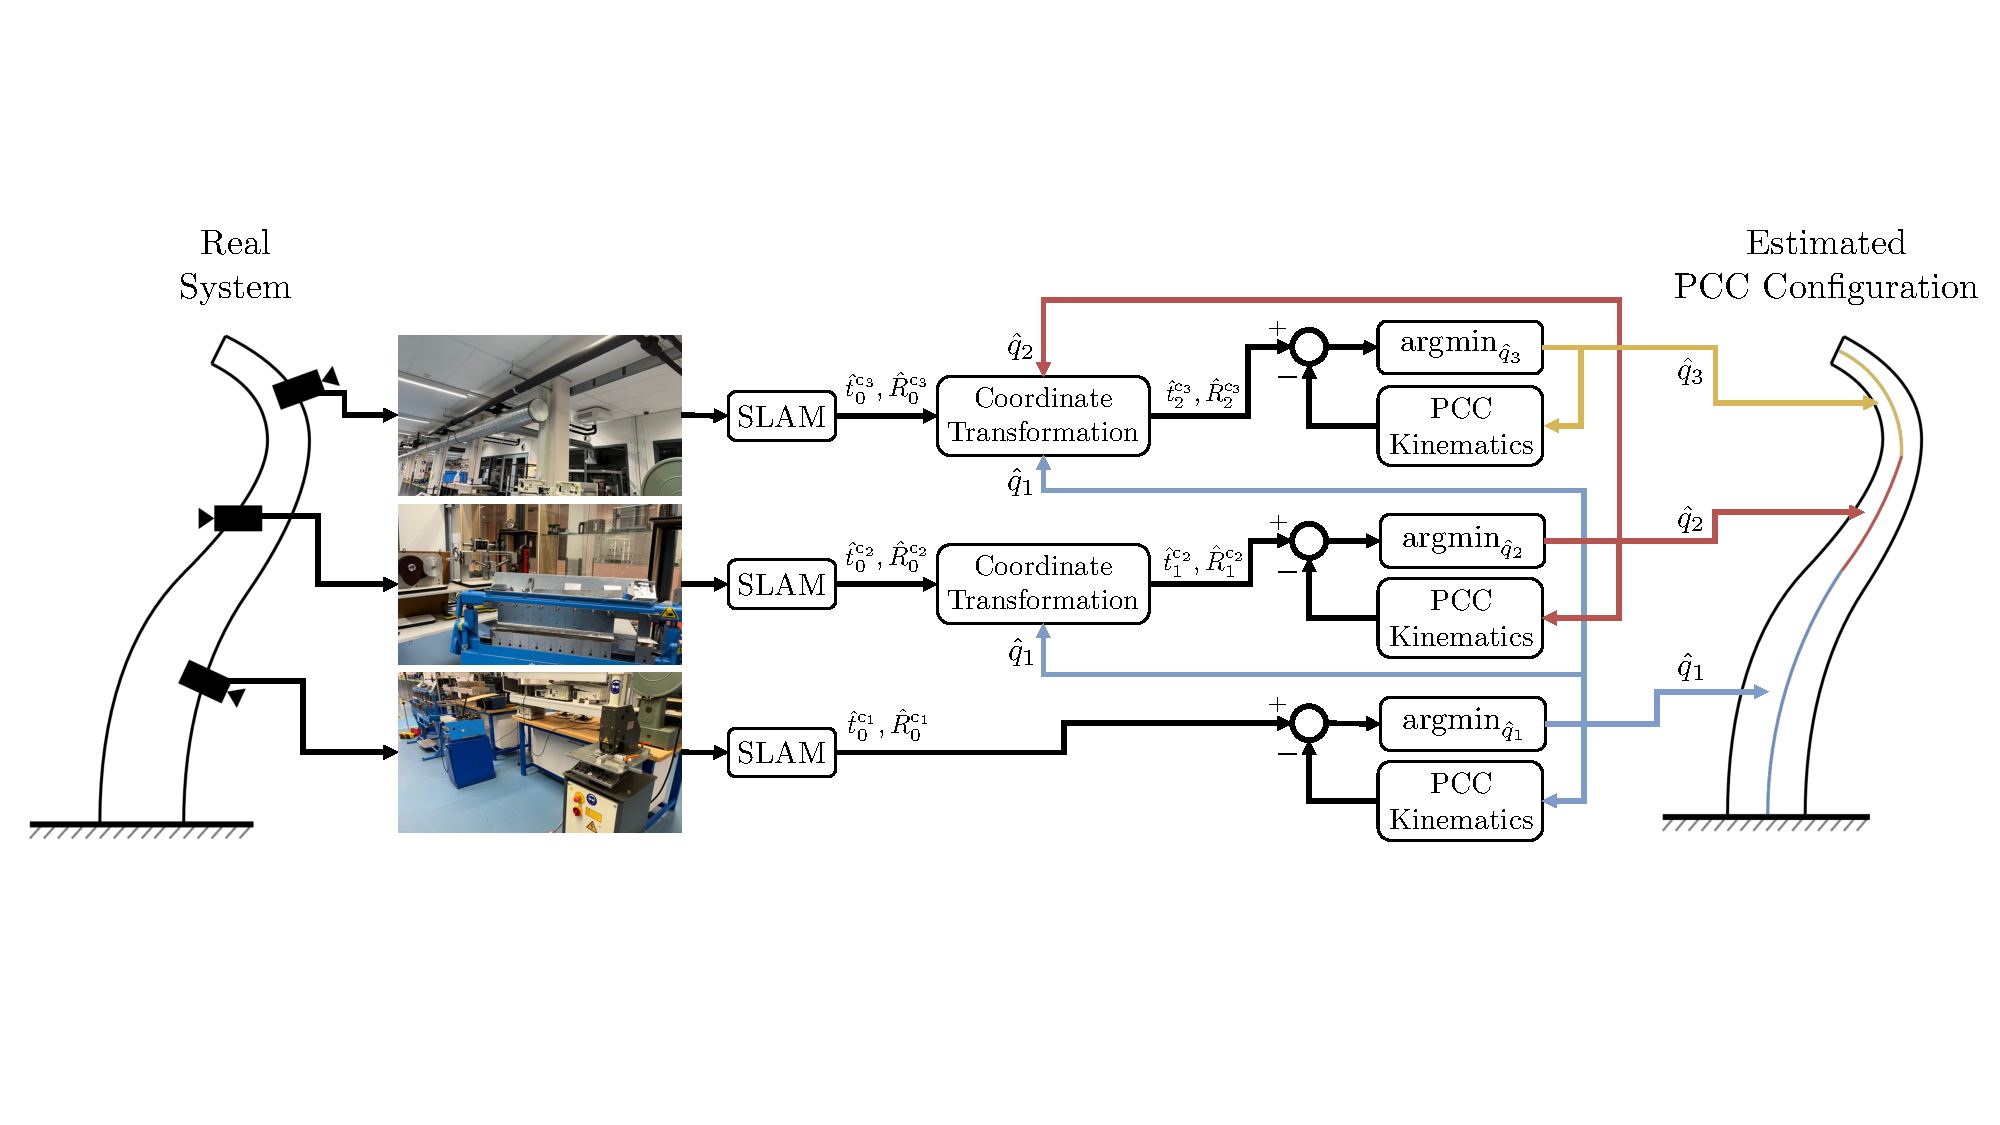
\includegraphics[width=0.69\columnwidth]{srslam/figures/graphic_method_overview_v5_cropped.pdf} \label{fig:srslam:method_overview}}
     \subfigure[Kinematics]{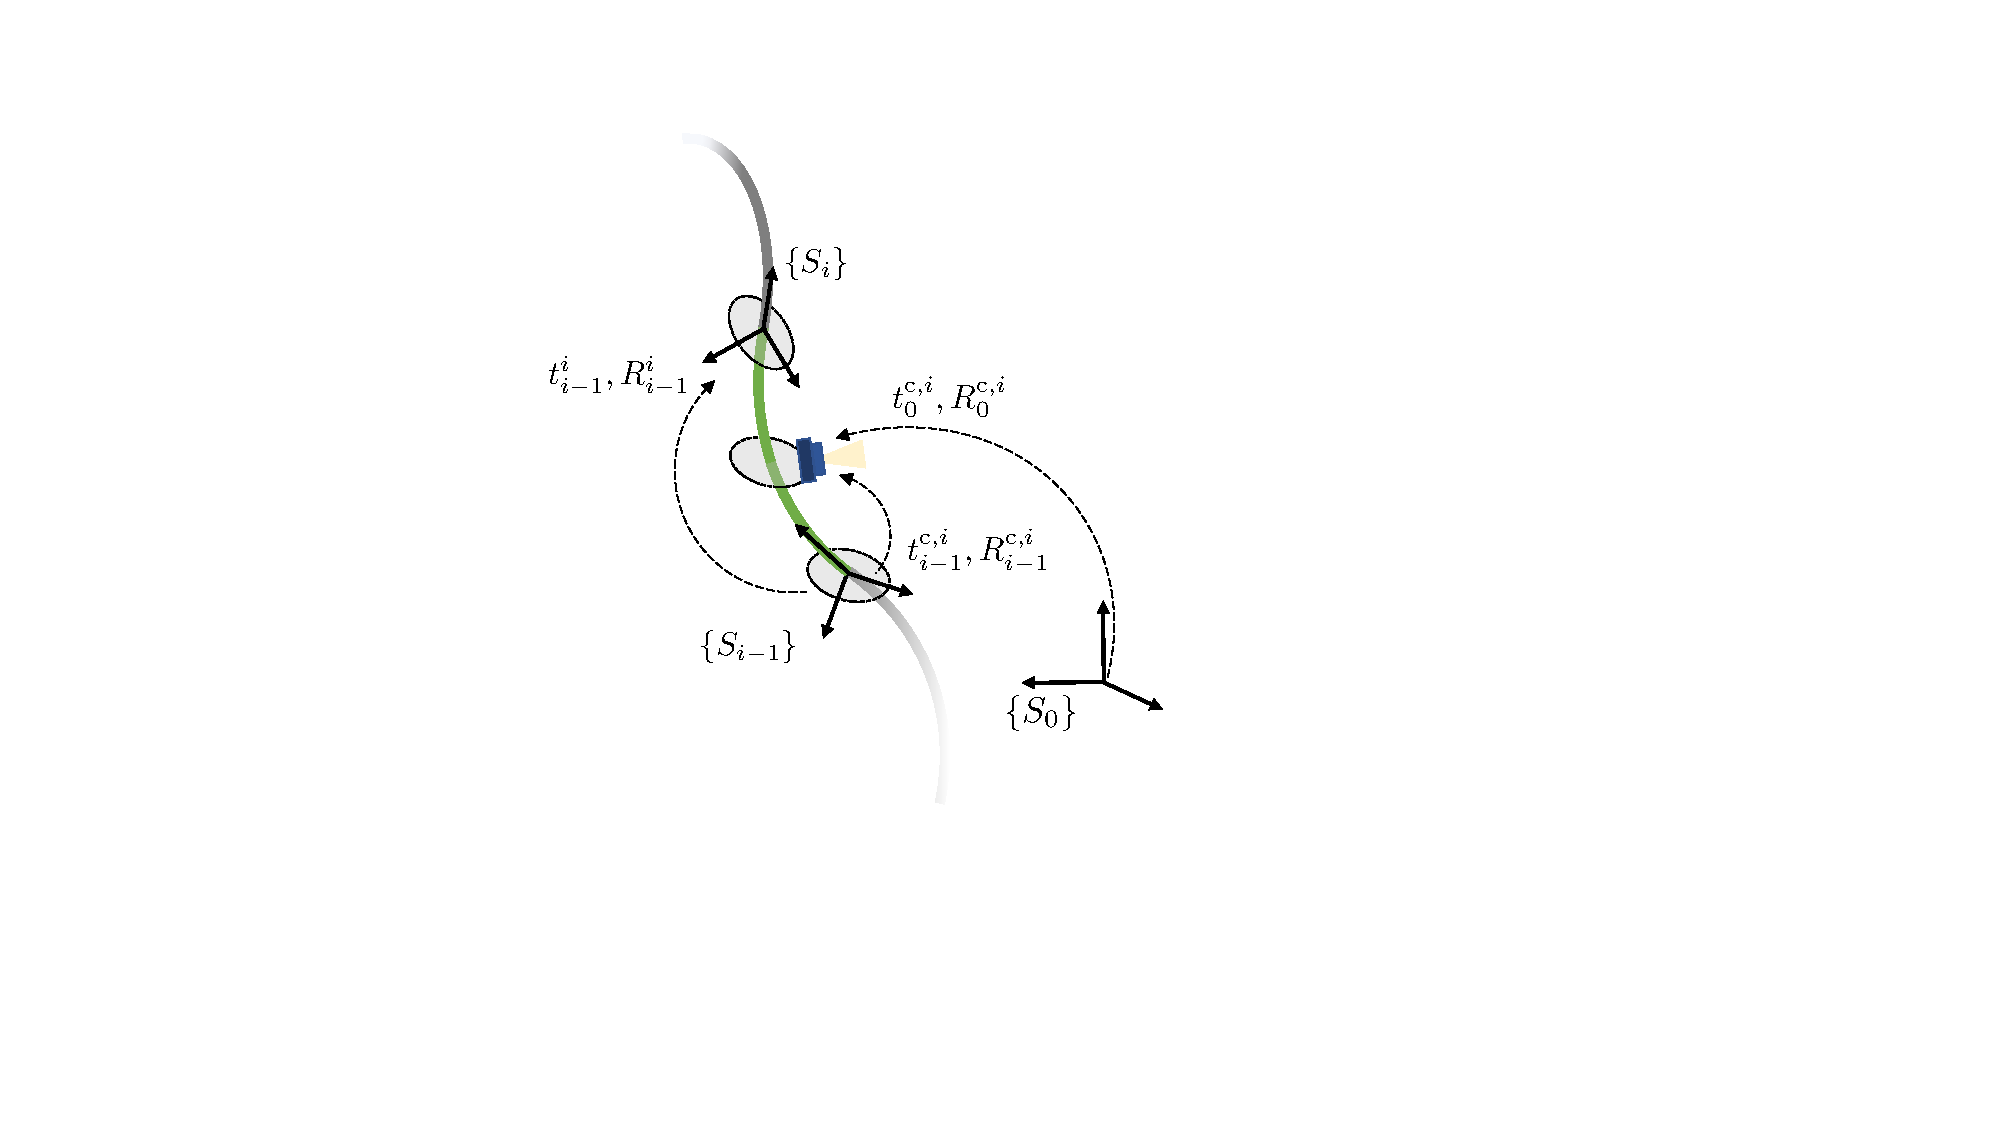
\includegraphics[width=0.24\columnwidth, trim = {0 0 0 0}, clip]{srslam/figures/kinematics_v2.pdf}\label{fig:srslam:kinematic_parameters} \label{fig:srslam:kinematics}}
     \caption{ Panel (a) shows a pictorial representation of the proposed perception strategy. Cameras are attached to a soft continuum robot. We propose to use ORB-SLAM~\cite{mur2017orb} to gather a pose estimate for each camera. The results are iteratively combined to extract local transformation, and refined by projecting the resulting postures onto the manifold of configurations attainable with the \gls{PCC} kinematics. The result is an estimation of the full shape within the selected kinematic description $\hat{q}$. Panel (b) reports the main quantities of the kinematic model of one segment. }
\end{figure*}
\section{Proposed architecture: Shape estimation with kinematics-aware SLAM}
\label{sec:srslam:pose_estimation}

In this work we propose to use \gls{SLAM} for proprioception of continuum soft robots. Common kinematic parametrizations for soft robots such as \gls{PCC}~\cite{webster2010design} or \gls{PCS}~\cite{renda2018discrete} model the soft arm to consist of multiple segments with independent kinematic state variables. 
In the following, we assume that the robot's model consists of $n_{\mathrm{S}}$ segments, and that a monocular camera is attached to each segment. We rely on a \gls{PCC} kinematic formulation. However, the proposed results can be directly generalized to the PCS case.
%
%We expect that there exists a constant coordinate transformation between the camera and one point along the center-line of the soft segment.
%
Our goal is to reconstruct the full shape (i.e., a configuration $q_i$ for each segment) of the soft robot from the stream of images recorded by the cameras.

Fig. \ref{fig:srslam:method_overview} shows an overview of the proposed architecture.
%
%Monocular \gls{SLAM} algorithms are able to estimate the pose of each camera as the robot arm follows a trajectory.
We use \gls{SLAM} algorithms such as monocular ORB-SLAM~\cite{mur2017orb} to estimate the pose of cameras attached to the soft robotic arm.  The pose estimation consists of 3D translation and rotations describing the relative camera movement from initial calibration to the current state ($\hat{t}_0^{\mathrm{c}_i},\hat{R}_0^{\mathrm{c}_i}$ in the figure). Then, the kinematic model is simultaneously used to refine the outputs of the SLAM and transform it to the desired estimation of the configurations ($\hat{q}_1,\hat{q}_3,\hat{q}_3$ in the figure). Starting from the base segment, and progressively iterating up until reaching the tip of the robot, we express translation and rotations in local coordinates, and we optimize the estimated configurations segment-by-segment starting at the proximal end by projecting the pose estimate into the 3D \gls{PCC} kinematics.
% This approach leverages known characteristics of the continuum soft robot and reduces the pose estimation error.

In the following subsections, we provide more details on the various components of this architecture.

\subsection{Background: Monocular ORB-SLAM}
We choose monocular ORB-SLAM~\cite{mur2017orb} for pose estimation of the camera locations. Although this technological solution has never been applied to soft robots, the algorithm itself is well established and its applications to mobile robotics widespread. As such, we  briefly describe here only the major steps of the algorithm.%, based on the pipeline in \ref{fig:srslam:algorithmpipeline}. 
 \begin{enumerate}
     \item \textbf{Map Initialization}: ORB-SLAM initializes a map of 3D points based on two video frames. The 3D points and relative camera pose are computed using triangulation of 2D ORB feature correspondences.
     \item \textbf{Tracking}: Once the map is initialized, the camera pose is estimated for each new frame by matching features in the current frame to features in the last key frame. The estimated camera pose is refined by tracking the local map.
     \item \textbf{Local Mapping}: If the current frame is identified as a key frame, it is used to create new 3D map points. At this stage, \gls{BA} is used to minimize re-projection errors by adjusting the camera pose and 3D points.
     \item \textbf{Loop Closure}: Loops are detected for each key frame by comparing it against all previous ones. % key frames using the bag-of-features approach~\cite{o2011introduction}. 
     %Any time a loop closure is detected, the pose graph is optimized to refine the camera poses of all the key frames.
     This information is used to optimize the poses.
 \end{enumerate}
An important aspect of \gls{SLAM} algorithms are key frames, which are a subset of video frames that contain cues for localization and tracking. Two consecutive key frames usually involve sufficient visual change. % In the end the algorithm returns the camera poses for each key frame.

\subsection{Projection into PCC-Kinematics}
Once the \gls{SLAM} algorithm provides us with the estimated camera poses, we want to interpret and correct them such as that they are coherent with the \gls{PCC} kinematic model.
%
In this paper, we consider the \emph{Delta} parametrization~\cite{della2020improved} of the \gls{PCC} kinematics, but the formulation could also be easily adapted to other kinematic parametrizations such as \gls{PCS}~\cite{renda2018discrete}.

% \begin{figure}[ht]
%     \centering
%     \includegraphics[width=1\columnwidth]{srslam/figures/kinematic_parameters.pdf}\label{fig:srslam:kinematic_parameters}
%     \\
%     \caption{One graphic showing the kinematic parameters for a multi-segment setup with multiple cameras and all used coordinate transformations.}
% \end{figure}

We show a pictorial representation of this kinematic model in Fig. \ref{fig:srslam:kinematics}. Each segment of original length $L_{0,i}$ is described with three configuration variables 
%
%\begin{equation}
    $q_i \in \mathbb{R}^{3} = \begin{pmatrix}\Delta_{x,i} & \Delta_{y,i} & \delta L_i\end{pmatrix}^\mathrm{T}$,
%\end{equation}
where $\delta L_i$ is segment's extension, and $\Delta_{x,i}$ and $\Delta_{y,i}$ are the differences of the arc lengths of the segment at a radial distance of $d_i$ from the center-line along both cardinal directions of the base~\cite{della2020improved}. The complete robot's configuration is $q \in \mathbb{R}^{3 n_{\mathrm{S}}}$. The coordinate transformation for segment $i$ from the base frame $\{ S_{i-1} \}$ into the tip frame $\{ S_{i} \}$ as a function of the configuration $q_i$ is given by~\cite{della2020improved}
\begin{equation}
\label{eq:srslam:transformation_improved_pcc}
\begin{split}
    R_{i-1}^{i} &= 
    \begin{pmatrix}
        1 + \frac{\Delta_{x,i}^2}{\Delta_{i}^2} \left ( \mathrm{c}_i - 1 \right ) & \frac{\Delta_{x,i} \Delta_{y,i}}{\Delta_{i}^2} \left ( \mathrm{c}_i - 1 \right ) & \frac{\Delta_{x,i}}{\Delta_i} \mathrm{s}_i\\
        \frac{\Delta_{x,i} \Delta_{y,i}}{\Delta_{i}^2} \left ( \mathrm{c}_i - 1 \right ) & 1 + \frac{\Delta_{y,i}^2}{\Delta_{i}^2} \left ( \mathrm{c}_i - 1 \right ) & \frac{\Delta_{y,i}}{\Delta_i} \mathrm{s}_i\\
        \frac{-\Delta_{x,i}}{\Delta_i} \mathrm{s}_i & \frac{-\Delta_{y,i}}{\Delta_i} \mathrm{s}_i & \mathrm{c}_i
    \end{pmatrix},\\
    \vspace{0.25em}
    t_{i-1}^{i} &= \frac{d_i ( L_{0,i}+\delta L_i)}{\Delta_i^2}
    \begin{pmatrix}
        \Delta_{x,i} (1 - \mathrm{c}_i) & \Delta_{y,i} (1 - \mathrm{c}_i) & \Delta_{i} \mathrm{s}_i
    \end{pmatrix}^{\mathrm{T}},
\end{split}
\end{equation}
where we substituted $\Delta_i = \sqrt{\Delta_{x,i}^2 + \Delta_{y,i}^2}$, $\mathrm{s}_i = \sin \left ( \frac{\Delta_i}{d_i} \right )$, and $\mathrm{c}_i = \cos \left ( \frac{\Delta_i}{d_i} \right )$ for conciseness.

We describe the coordinate frame of camera $i$ with $\{ S_{\mathrm{c}_i} \}$. It is assumed that there exists a fixed transformation $T_{\check{\mathrm{c}},i}^{\mathrm{c}_i} \in \mathbb{R}^{4 \times 4}$ from frame $\{ S_{\check{\mathrm{c}},i} \}$ to the camera frame $\{ S_{\mathrm{c}_i} \}$. 
$\{ S_{\check{\mathrm{c}},i} \}$ is localized at a distance $l_{\mathrm{c}_i}$ along the center-line from the base of segment $i$. 
The transformation $T_{i-1}^{\check{\mathrm{c}},i}(q_{\check{c},i})$ from the base to the frame $\{ S_{\check{\mathrm{c}},i} \}$ can be found with \eqref{eq:srslam:transformation_improved_pcc} by plugging in the adjusted configuration $q_{\check{c},i}$ defined as
\begin{equation}\label{eq:srslam:camera_configuration}
    q_{\check{c},i} = \frac{l_{\mathrm{c}_i}}{L_{0,i}} q_i,
\end{equation}
and the adjusted original length  $l_{\mathrm{c}_i}$.

The \gls{SLAM} algorithm provides a pose estimate for the translation $\hat{t}_{\mathrm{c},\mathrm{t}0,i}^{\mathrm{c}_i} \in \mathbb{R}^3$ and rotation $\hat{R}_{\mathrm{c},\mathrm{t}0,i}^{\mathrm{c}_i} \in \mathbb{R}^{3 \times 3}$ relative to the known initial reference frame of the camera $\{ S_{\mathrm{c},\mathrm{t}0,i} \}$. 
Thus, we first transform the pose estimates to the inertial frame of the robot $\{ S_0 \}$
\begin{equation}
    \begin{pmatrix}
        \hat{t}_{0}^{\mathrm{c}_i}\\
        1
    \end{pmatrix}
    = T_0^{\mathrm{c},\mathrm{t}0,i}
    \begin{pmatrix}
        \hat{t}_{\mathrm{c},\mathrm{t}0,i}^{\mathrm{c}_i}\\
        1
    \end{pmatrix},
    \quad
    \hat{R}_{0}^{\mathrm{c}_i} = R_0^{\mathrm{c},\mathrm{t}0,i} \hat{R}_{\mathrm{c},\mathrm{t}0,i}^{\mathrm{c}_i}.
\end{equation}

We introduce the following notations for the \gls{PCC} kinematics
\begin{equation}\label{eq:srslam:Pi}
\begin{split}
    \hat{t}_{i-1}^{\mathrm{c}_i} &= \Pi_\mathrm{t}(\hat{q}_i) = 
    \hat{T}_{i-1}^{\check{\mathrm{c}},i} \left (\frac{l_{\mathrm{c}_i}}{L_{0,i}} \hat{q}_i \right )
    t_{\check{\mathrm{c}},i}^{\mathrm{c}_i}\\
    \hat{R}_{i-1}^{\mathrm{c}_i} &= \Pi_\mathrm{R}(\hat{q}_i) =
    \hat{R}_{i-1}^{\check{\mathrm{c}},i} \left (\frac{l_{\mathrm{c}_i}}{L_{0,i}} \hat{q}_i \right )
    R_{\check{\mathrm{c}},i}^{\mathrm{c}_i},
\end{split}
\end{equation}
where $\hat{t}_{i-1}^{\check{\mathrm{c}},i}$ and $\hat{R}_{i-1}^{\check{\mathrm{c}},i}$ describe the translation and rotation from the base of the segment to the camera frame according to the \gls{PCC} kinematic model for an estimated configuration of the the segment $\hat{q}_i$. $\hat{T}_{i-1}^{\check{\mathrm{c}},i}(q_{\check{c},i})$ and $\hat{R}_{i-1}^{\check{\mathrm{c}},i}(q_{\check{c},i})$ are based on \eqref{eq:srslam:transformation_improved_pcc} and a function of the adjusted configuration $q_{\check{c},i}$ referenced in \eqref{eq:srslam:camera_configuration}.

Additionally, the pose estimates by the \gls{SLAM} algorithm need to be transformed to the base frame of segment $i$. Thus, we introduce the following
\begin{equation}\label{eq:srslam:Psi}
\begin{split}
    \hat{t}_{i-1}^{\mathrm{c}_i} &= \Psi_\mathrm{t}(q_1 \dots q_{i-1}, \hat{t}_{0}^{\mathrm{c}_i}) =
    \prod_{\tilde{i}=1}^{i-1} \left ( T_{\tilde{i}-1}^{\tilde{i}} \left (\hat{q}_{\tilde{i}} \right )  \right )^\mathrm{T}
    \begin{pmatrix}
        \hat{t}_{0}^{\mathrm{c}_i}\\
        1
    \end{pmatrix},\\
    \hat{R}_{i-1}^{\mathrm{c}_i} &= \Psi_\mathrm{R}(q_1 \dots q_{i-1}, \hat{R}_{0}^{\mathrm{c}_i}) =
    \prod_{\tilde{i}=1}^{i-1} \left ( R_{\tilde{i}-1}^{\tilde{i}} \left (\hat{q}_{\tilde{i}} \right )  \right )^\mathrm{T}
    \hat{R}_{0}^{\mathrm{c}_i}.
\end{split}    
\end{equation}

Next, we define a cost function to optimize the pose estimate by projecting them into the \gls{PCC}-kinematics
% Please note, that we do not include the orientation estimate $\hat{R}_{0}^{\mathrm{c}_i}$ by the \gls{SLAM} algorithm in the cost function.
%
\begin{equation}\label{eq:srslam:cost_fun}
    \min_{\hat{q}} \sum_{i=1}^{n_\mathrm{S}} f_{\mathrm{t},i}(\hat{q}) + \lambda_\mathrm{R} f_{\mathrm{R},i}(\hat{q}),
\end{equation}
with
\begin{equation}\label{eq:srslam:cost_fun_ingredients}
\begin{split}
    f_{\mathrm{t},i}(\hat{q}) &=
    \big\lVert 
    \Pi_\mathrm{t}(\hat{q}_i) - \Psi_\mathrm{t}(q_1 \dots q_{i-1}, \hat{t}_{0}^{\mathrm{c}_i})
    \big\rVert_2,\\
    f_{\mathrm{R},i}(\hat{q}) &=
    \big\lVert 
    \Pi_\mathrm{R}(\hat{q}_i) - \Psi_\mathrm{R}(q_1 \dots q_{i-1}, \hat{R}_{0}^{\mathrm{c}_i})
    \big\rVert_F,
\end{split}
\end{equation}
where the Euclidean norm is used to compute the translational error between the predicted translation by the \gls{PCC} kinematic model and the estimated translation by \gls{SLAM}. The rotational error is weighted with $\lambda_\mathrm{R}$ and computed with the Frobenius norm between the predicted rotation matrix by the \gls{PCC} kinematics and the estimated orientation by \gls{SLAM} represented as a rotation matrix as well.

Please note, that the optimization of the configuration estimate $\hat{q}$ can be decoupled for each segment. 
We start by optimizing the configuration of the first segment $\hat{q}_1$ based on $\Psi_\mathrm{t}(\hat{t}_{0}^{\mathrm{c},1})$ and $\Psi_\mathrm{R}(\hat{R}_{0}^{\mathrm{c},1})$. Next, we optimize the configuration of the second segment $\hat{q}_2$ taking into account the already optimized configuration of segment one in $\Psi_\mathrm{t}(\hat{q}_1, \hat{t}_{0}^{\mathrm{c},2})$ and $\Psi_\mathrm{R}(\hat{q}_1, \hat{R}_{0}^{\mathrm{c},2})$. 
Subsequently, we move on to optimize the remaining segments sequentially as described by Algorithm~\ref{alg:srslampose_estimation}. This procedure is also graphically represented by the right side of Fig. \ref{fig:srslam:method_overview}.

\begin{algorithm}[hbt!]
\caption{Pose estimation for soft robots through SLAM}\label{alg:srslampose_estimation}
\begin{algorithmic}
\REQUIRE $o \in \mathbb{R}^{n_\mathrm{S}}$ \COMMENT{Observations of all cameras}
\ENSURE $\hat{q} \in \mathbb{R}^{3 n_\mathrm{S}}$ \COMMENT{Estimated robot configuration}
\STATE $i \gets 1$
\WHILE{$i \leq n_\mathrm{S}$}
    \vspace{0.25em}
    \STATE $\hat{t}_{0}^{\mathrm{c}_i} \gets T_0^{\mathrm{c},\mathrm{t}0,i} \: \mathrm{SLAM}_\mathrm{t}(o_i)$ \COMMENT{Translational est. SLAM}
    \vspace{0.25em}
    \STATE $\hat{R}_{0}^{\mathrm{c}_i} \gets R_0^{\mathrm{c},\mathrm{t}0,i} \: \mathrm{SLAM}_\mathrm{R}(o_i)$ \COMMENT{Rotational est. SLAM}
    \vspace{0.25em}
    \STATE $f_{\mathrm{t},i}(\hat{q}) \gets
    \big\lVert 
    \Pi_\mathrm{t}(\hat{q}_i) - \Psi_\mathrm{t}(q_1 \dots q_{i-1}, \hat{t}_{0}^{\mathrm{c}_i})
    \big\rVert_2$
    \vspace{0.25em}
    \STATE $f_{\mathrm{R},i}(\hat{q}) \gets
    \big\lVert 
    \Pi_\mathrm{R}(\hat{q}_i) - \Psi_\mathrm{R}(q_1 \dots q_{i-1}, \hat{R}_{0}^{\mathrm{c}_i})
    \big\rVert_F$
    \vspace{0.25em}
    \STATE $f_{c,i}(\hat{q}) \gets f_{\mathrm{t},i}(\hat{q}) + \lambda_\mathrm{R} f_{\mathrm{R},i}(\hat{q})$ \COMMENT{Cost function for $\hat{q}_i$}
    \vspace{0.25em}
    \STATE $\hat{q}_i \gets \argmin_{\hat{q_i}} f_c(\hat{q})$
    \vspace{0.25em}
    \STATE $i \gets i + 1$
\ENDWHILE
\end{algorithmic}
\end{algorithm}

\section{Simulations}
\label{sec:srslam:simulations}

We quantitatively evaluate our approach in simulation for one soft robotic segment with a camera attached to the tip of the robot. 
We first compute trajectories that behave according to \gls{PCC} kinematics. 
Next, we render photo-realistic images for the camera attached to the tip of the segment for every time step using a virtual environment implemented in Blender. Subsequently, we process the synthetic camera images with the ORB-SLAM~\cite{mur2017orb} algorithm and projected the estimated poses of the tip of the segment into the \gls{PCC} kinematic model as outlined in Section~\ref{sec:srslam:pose_estimation}. Finally, we compare the estimated poses against the ground truth and statistically evaluate the \gls{RMSE} both for translational and rotational estimates. More details follow.

\subsection{System}\label{sub:srslam:simulations_system}
We consider a soft robotic segment of diameter \SI{20}{mm} diameter and with varying lengths $L_{0,1}$ between \SI{15}{cm} and \SI{100}{cm}.
As the camera is attached to the tip of the segment, we set $l_{\mathrm{c}_1} = L_{0,1}$ and define $T_{\check{\mathrm{c}},1}^{\mathrm{c},1} = \mathbb{I}^4$.

\subsection{Trajectories and calibration sequence}\label{sub:srslam:trajectories}
Three different trajectories are considered for the simulated movement of the soft robotic segment and its attached virtual camera. While the first one represents a planar side bending, the second one describes an “8” shape with the tip, and the last one covers a lobe of the “8”. 
Those trajectories were commanded in $\Delta_{x,1}$ and $\Delta_{y,1}$, with the following mathematical formulas:
\begin{equation}\label{eq:srslam:trajectory_parametrization}
    \Delta_{x,1} = L_{0,1} A_x \sin(2 \pi f_x) \qquad \Delta_{y,1} = L_{0,1} A_y \sin(2 \pi f_y),
\end{equation}
with $L_{0,1}$ the unextended length of the robot, $A_x$ and $A_y$ amplitudes of the sinusoids and $f_x$ and $f_y$ frequencies of the sinusoids.
The parameters $f_x$ and $f_y$ are defined as follows with $k$ representing the current time index:
\begin{equation}
    f_x = \frac{F_x (k-1)}{n_{\mathrm{t}}}, \qquad f_y = \frac{F_y (k-1)}{n_{\mathrm{t}}}.
\end{equation}
Please note that these trajectories do not contain any segment elongation. 
We list the chosen amplitudes and frequencies of the trajectories in Table~\ref{tab:srslam:trajectory_params}. Each trajectory is generated considering different robot lengths, namely \SI{15}{cm}, \SI{30}{cm} and \SI{100}{cm}. The number of time steps $n_{\mathrm{t}}$ is chosen at $120$. 
The commanding of $\Delta_{x,1}$ and $\Delta_{y,1}$ is such that the amplitude and frequency of the trajectory are independent of the number of frames (i.e., time steps).
In Figure~\ref{fig:srslam:trajectories}, we show a 3D visualization of the trajectories corresponding to a segment length of \SI{15}{cm}.

\begin{table}
\centering
\caption{Parameters of the implemented trajectories. We list the amplitudes and the frequencies of the trajectories parametrized by $\Delta_{x,1}$ and $\Delta_{y,1}$ as specified in \eqref{eq:srslam:trajectory_parametrization}.}
% \begin{scriptsize}
\begin{tabular}{lcccc}\toprule
\textbf{Trajectory} & $A_x$ & $A_y$ & $F_x$ & $F_y$\\
\midrule
Trajectory 1: planar side bending & 0.1 & 0 & 0.5 & 0\\
Trajectory 2: half 8-shape & 0.05 & 0.05 & 1 & 0.5\\
Trajectory 3: full 8-shape & 0.05 & 0.05 & 2 & 1\\
\bottomrule
\end{tabular}
% \end{scriptsize}
\label{tab:srslam:trajectory_params}
\end{table}

\begin{figure*}[ht]
  \centering
  \subfigure[Trajectory 1]{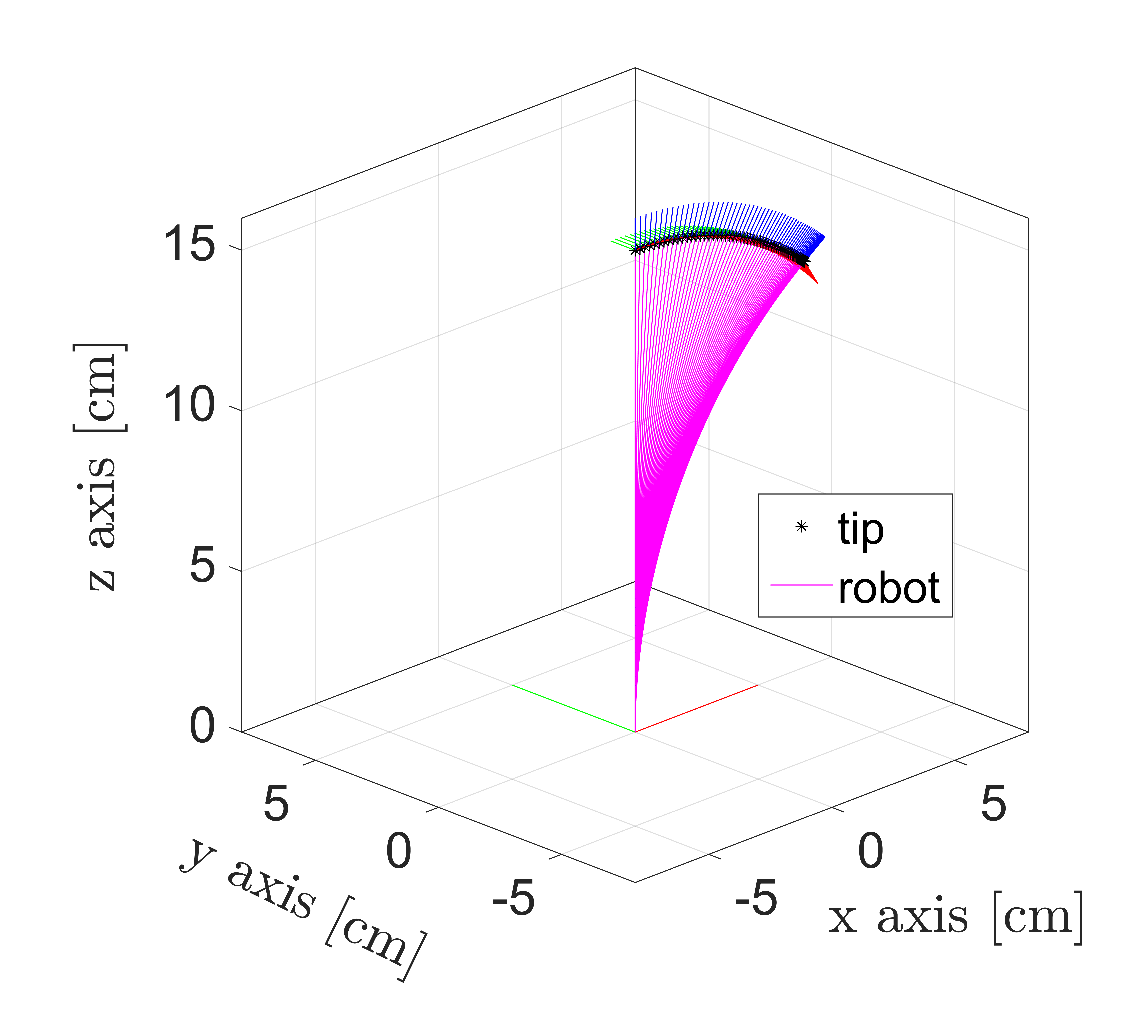
\includegraphics[width=0.21\textwidth]{srslam/figures/t1_l15_v3.0.eps}\label{fig:srslam:traj1}}
  \hspace{0.005\textwidth}% \hfill% or \hspace{5mm} or \hspace{0.3\textwidth}
  \subfigure[Trajectory 2]{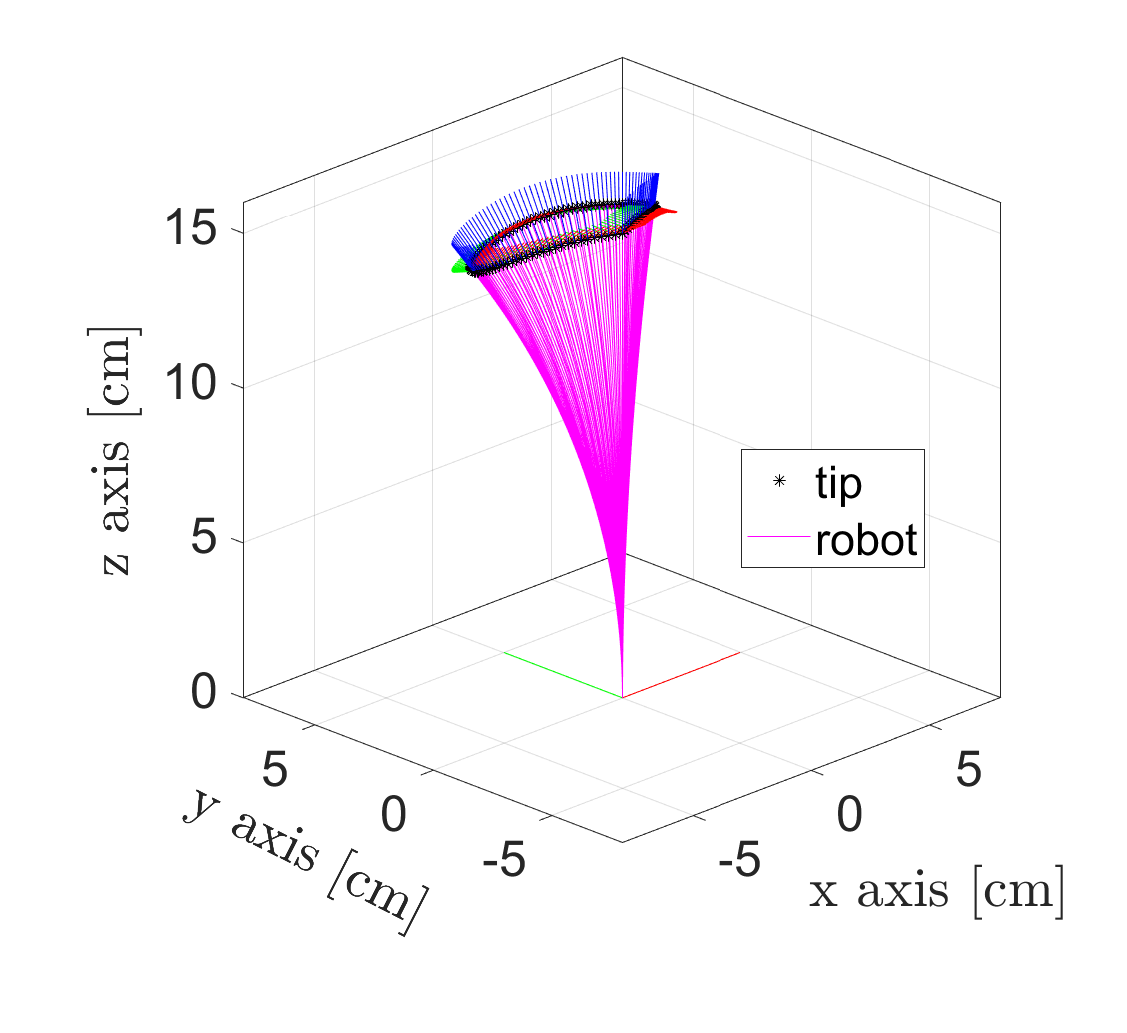
\includegraphics[width=0.21\textwidth]{srslam/figures/t2_l15_v3.2.eps}\label{fig:srslam:traj2}}\hspace{0.005\textwidth}% \hfill% or \hspace{5mm} or \hspace{0.3\textwidth}
  \subfigure[Trajectory 3]{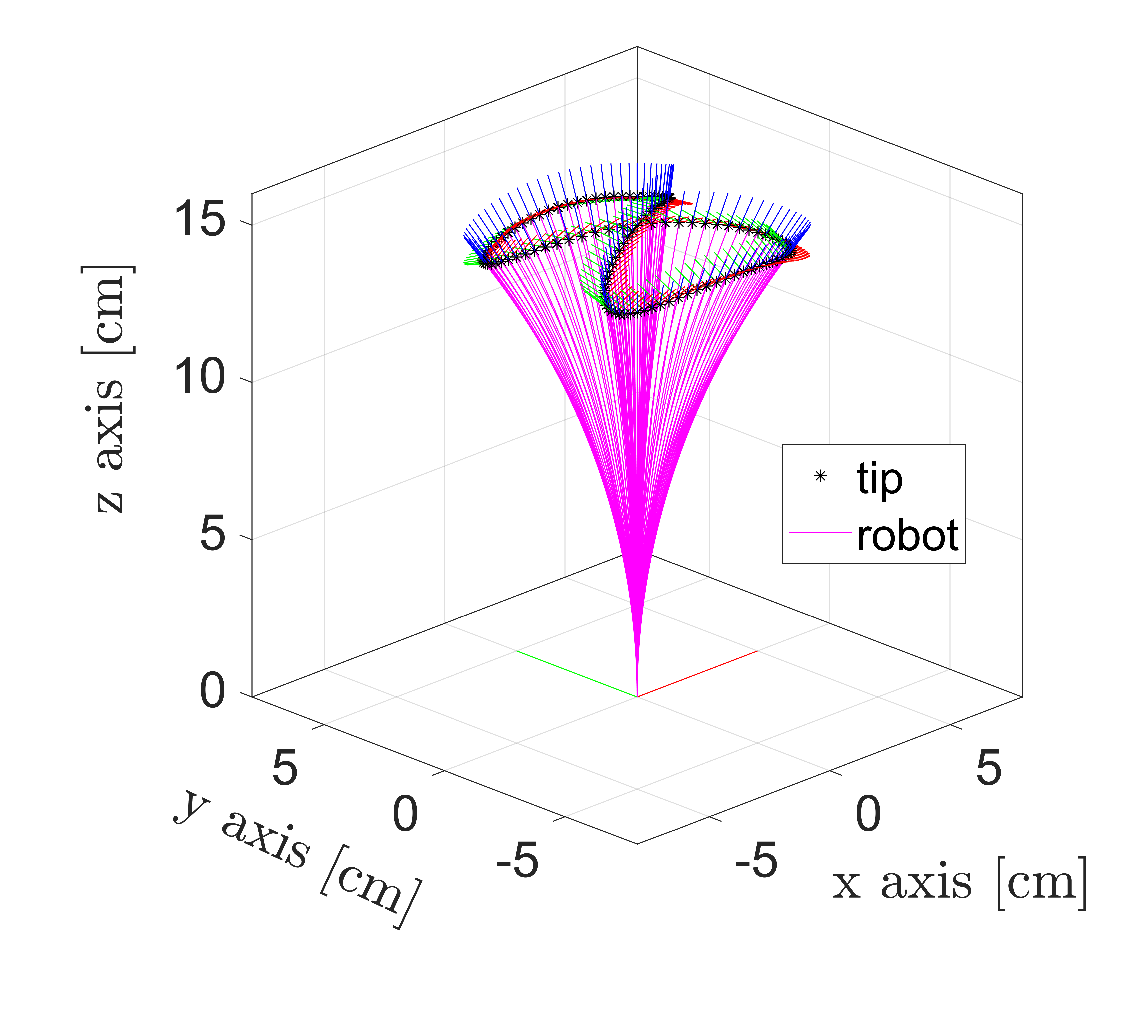
\includegraphics[width=0.21\textwidth]{srslam/figures/t3_l15_v3.1.eps}\label{fig:srslam:traj3}}\hfill
  \subfigure[Virtual interior scene]{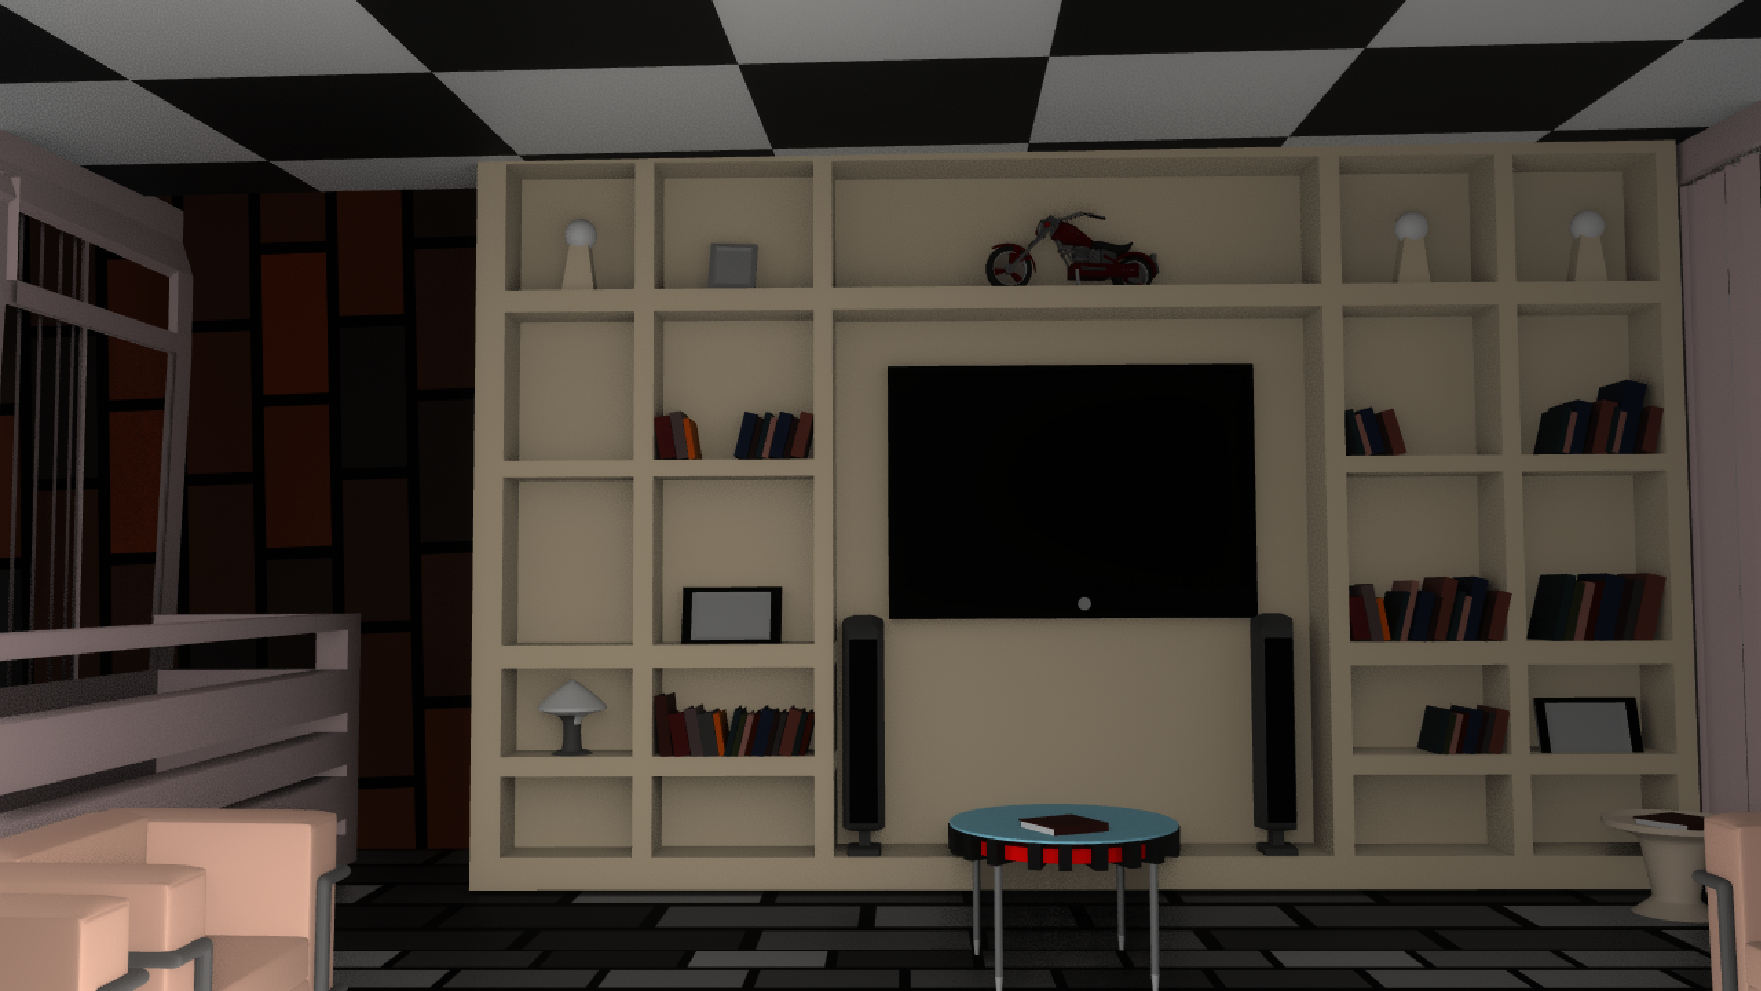
\includegraphics[width=0.3\textwidth]{srslam/figures/interior_scene.pdf}\label{fig:srslam:interior_scene}}
  \caption{3D visualization of the three trajectories used in our simulations and experiments for a segment with \SI{15}{cm} length. In magenta, we visualize the trajectory of the full robot, and in black, the tip positions. Additionally, the tip orientation (red = x-axis, green = y-axis, blue = z-axis) is displayed. The virtual interior scene used for the Blender renderings is presented in the last column.}
  \label{fig:srslam:trajectories}
\end{figure*}

In addition to the robot trajectory, a calibration sequence trajectory is designed to initialize the \gls{SLAM} map. 
It is good practice to move the camera parallel to the scene captured. Accordingly, we decide to move the camera into the $x$ cardinal direction of the segment base frame with the translation distance proportional to the robot length.

\subsection{Rendering of synthetic images}
The rendering software Blender allows us, among other things, to load a 3D model of the environment, follow customized trajectories with a virtual camera, and render photo-realistic synthetic pictures of the environment from the chosen camera perspective. We use an interior scene published by \href{https://www.nextwavemultimedia.com/html/3dblendermodel.html}{Nextwave Multimedia}. We report a view of the scene in Fig. \ref{fig:srslam:interior_scene}.
The virtual camera is set to be perspective with a focal length of \SI{30}{mm}.
For each run, we randomly initialize the trajectory at one of seven predefined launch points in the indoor environment to diversify the coverage of the environment.
The x-, y-, and z-coordinates of the seven initial positions have a standard deviation of \SI{0.5}{m}, \SI{0.2}{m}, \SI{0.4}{m} respectively. The initial orientation represented in XYZ Euler angles varies with a standard deviation of \SI{0.05}{rad}, \SI{0.13}{rad}, and \SI{1.17}{rad}.
For each trajectory, we render $120$ synthetic images along the trajectory and save them to a folder for later offline processing by the ORB-SLAM~\cite{mur2017orb} algorithm. Fig. \ref{fig:srslam:sequences_of_stills_simulations_cropped} reports a few representative stills of what the robot sees during one execution of the three trajectories discussed above.

\begin{figure*}
    \centering
    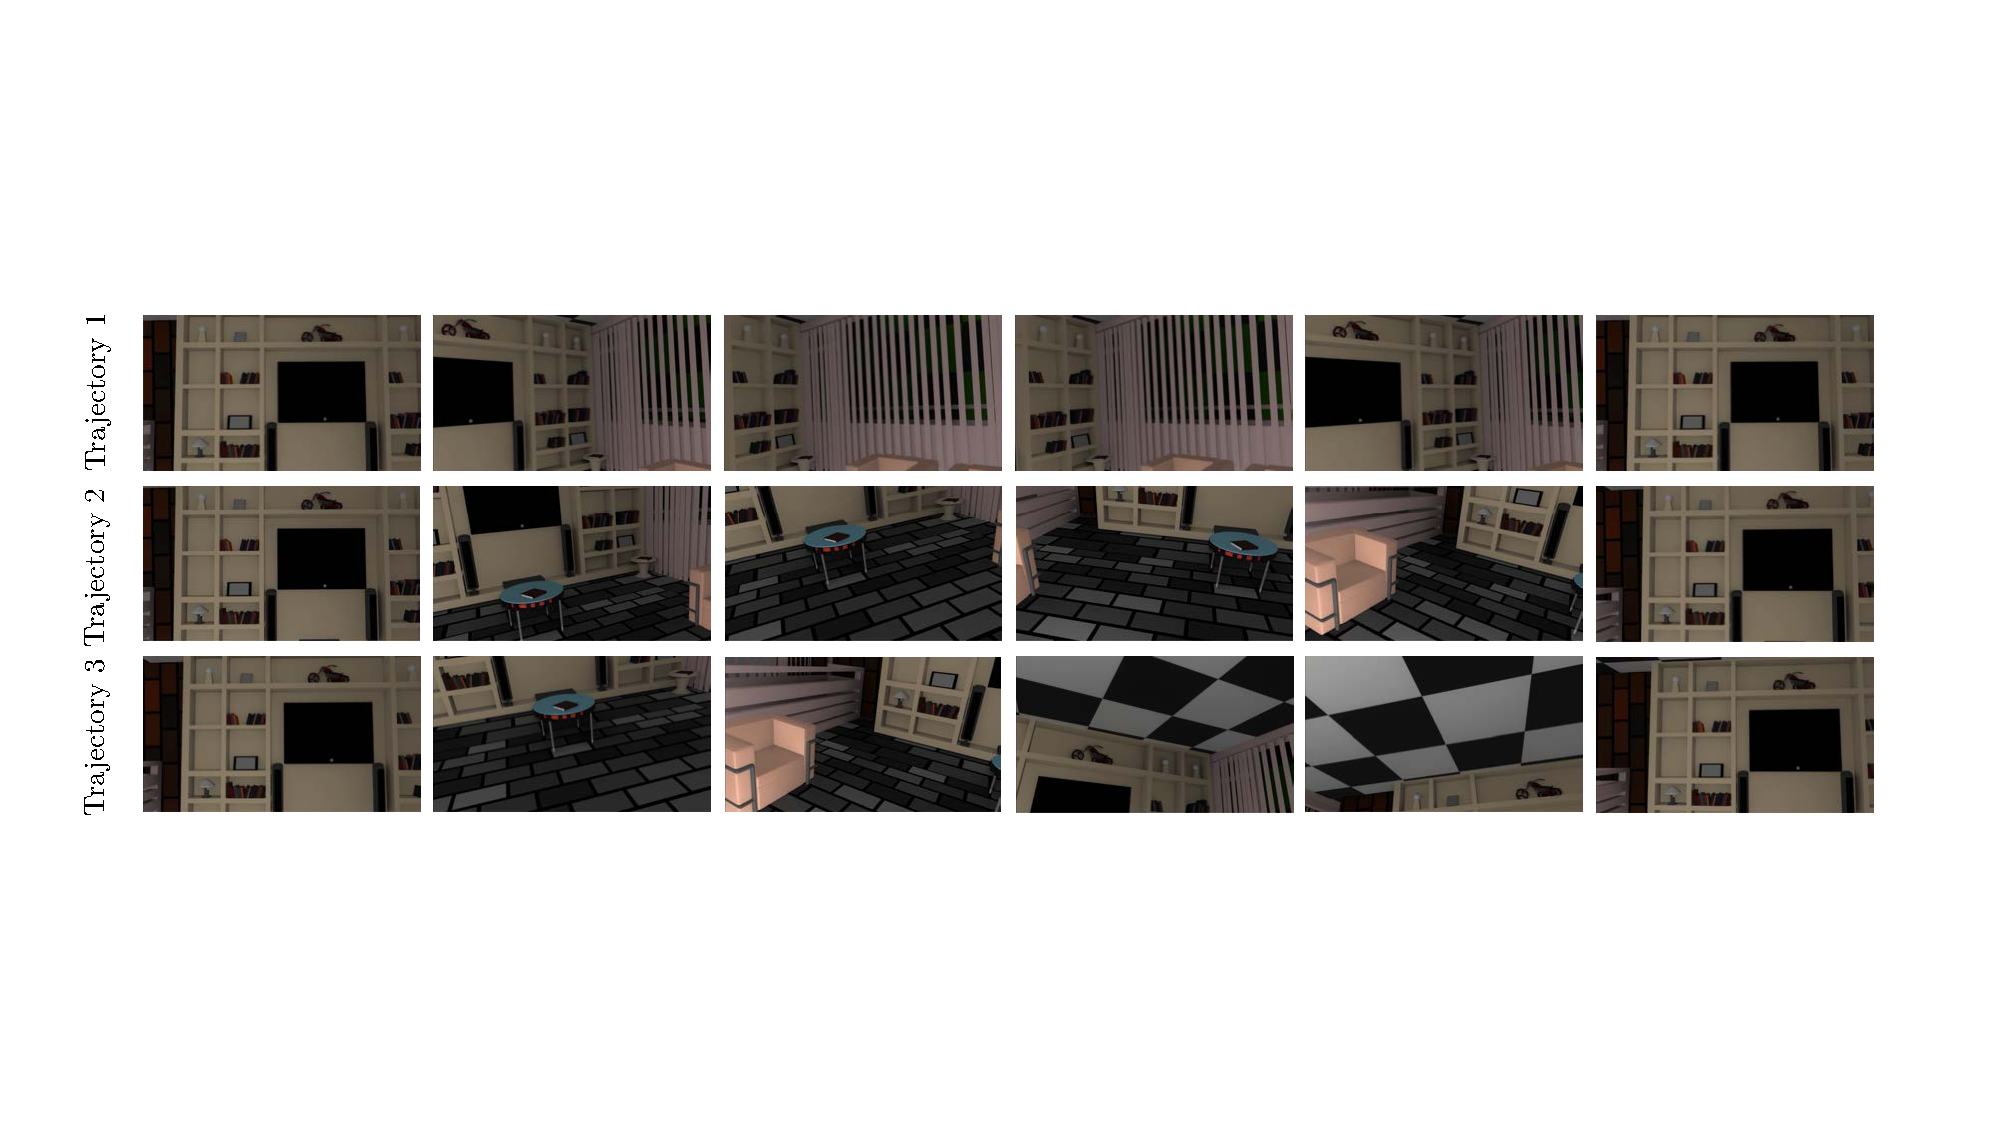
\includegraphics[width=0.9\textwidth]{srslam/figures/graphic_sequences_of_stills_simulations_compressed.pdf}
    \caption{Sequence of stills showing the rendered images by the virtual camera in Blender for three different trajectories and a robot segment of length \SI{15}{cm}. The trajectories are visualized in Figure~\ref{fig:srslam:trajectories}.}
    \label{fig:srslam:sequences_of_stills_simulations_cropped}
\end{figure*}

\subsection{Implementation of ORB-SLAM}
The synthetic images along the trajectory are processed offline by the ORB-SLAM~\cite{mur2017orb} algorithm. We rely on the official MATLAB implementation of ORB-SLAM. While we run our simulations offline to decouple any delays by the rendering and/or \gls{SLAM} pipeline, we would like to point out that other ORB-SLAM implementations, such as, for example, in C++, are able to be run in real-time at frame rates of between \SI{10}{Hz} to \SI{30}{Hz}~\cite{mur2017orb}.

\subsection{Projection into PCC kinematics}
The trade-off parameter $\lambda_\mathrm{R}$ between the rotational and the translational error in the cost function \eqref{eq:srslam:cost_fun} was manually tuned and set to $\lambda_\mathrm{R}=0.4$.
As the simulations do not contain any elongations of the segment, we set $\delta L_1 = 0$ in \eqref{eq:srslam:transformation_improved_pcc}. 
We solve the optimization problem outlined in \eqref{eq:srslam:cost_fun} using nonlinear least-squares with the Levenberg-Marquardt solver~\cite{levenberg1944method, marquardt1963algorithm} implemented in MATLAB as \emph{lsqnonlin}.

\subsection{Evaluation metrics}
To quantitatively evaluate the performance of our proposed approach, we introduce error metrics for both the translation and orientation estimates.
%
We measure the translational pose prediction error with a relative \gls{RMSE} $e_\mathrm{t}$
\begin{equation}\label{eq:srslam:evaluation_translational_error}
    e_\mathrm{t} = \frac{\sqrt{\sum_{t=1}^{n_\mathrm{t}} \left (\lVert \hat{t}_{0,t}^{\mathrm{c},1} - t_{0,t}^{\mathrm{c},1} \rVert_2 \right )^2}}{\sqrt{n_\mathrm{t}} \; l_\mathrm{traj}},
\end{equation}
where $l_\mathrm{traj}$ corresponds to the length of the trajectory and $n_\mathrm{t}$ the total number of data points along the trajectory. Similarly, we leverage the Frobenius norm for the rotational error $e_\mathrm{R}$
\begin{equation}\label{eq:srslam:evaluation_rotational_error}
    e_\mathrm{R} = \sqrt{\sum_{t=1}^{n_\mathrm{t}} \frac{\left (\big\lVert \hat{R}_{0,t}^{\mathrm{c},1} - R_{0,t}^{\mathrm{c},1} \big\rVert_F \right )^2}{n_\mathrm{t}}}.
\end{equation}
As torsion can often be neglected for soft robotic arms, we state the angle error for the orientation of the local z-axis of the tip of the segment for intuitive analysis of the orientation estimates. First, the unit vector of the local z-axis $\{ o_{1} \}_{0}$ is computed in the base frame $\{ S_0 \}$
\begin{equation}
    \{ o_1 \}_0 = R_{0,t}^{1}\begin{pmatrix}0 & 0 & 1\end{pmatrix}^\mathrm{T},
    \quad
    \{ \hat{o}_1 \}_0 = \hat{R}_{0,t}^{1}\begin{pmatrix}0 & 0 & 1\end{pmatrix}^\mathrm{T},
\end{equation}
which allows us to subsequently compute the angle error between the ground-truth z-axis of the tip $\{ o_1 \}_0$ and the estimated z-axis $ \{ \hat{o}_1 \}_0$
\begin{equation}\label{eq:srslam:evaluation_angle_error}
    e_{\theta_z} = \sqrt{\sum_{t=1}^{n_\mathrm{t}} \frac{\left (\arccos \left ( \{ o_1 \}_0 \cdot \{ \hat{o}_1 \}_0 \right ) \right )^2}{n_\mathrm{t}}}.
\end{equation}

\subsection{Results}\label{sub:srslam:simulation_results}
% \begingroup
% \setlength{\tabcolsep}{2.0pt} % Default value: 6pt
% \renewcommand{\arraystretch}{1} % Default value: 1
\begin{table*}
\centering
\caption{Relative \gls{RMSE} [\%] for translations as referenced in \eqref{eq:srslam:evaluation_translational_error} of various trajectories and of robot segments with different lengths (\SI{15}{cm}, \SI{30}{cm}, \SI{100}{cm}). We state the error as $\text{mean} \pm \text{stdev} \; (\min, \max)$ and compute the statistics over seven trials from different initial poses.}
\begin{tabular}{cclll}\toprule
\textbf{Trajectory} & \textbf{Optimization} & $L_{0,1} = \SI{15}{cm}$ & $L_{0,1} = \SI{30}{cm}$ & $L_{0,1} = \SI{100}{cm}$\\
\midrule
Trajectory 1 & No & $9 \pm 3 \; (5, 12)$ & $7 \pm 3 \; (3, 13)$ & $3 \pm 2 \; (1, 7)$ \\
Trajectory 1 & Yes & $0.4 \pm 0.2 \; (0.3, 0.8)$ & $2 \pm 1 \; (0, 4)$ & $1.0 \pm 0.7 \; (0.5, 2.3)$ \\
\midrule
Trajectory 2 & No & $9 \pm 4 \; (4, 17)$ & $6 \pm 2 \; (3, 8)$ & $1.9 \pm 0.9 \; (1.0, 3.0)$ \\
Trajectory 2 & Yes & $0.7 \pm 0.7 \; (0.3, 1.8)$ & $0.7 \pm 0.4 \; (0.2, 1.2)$ & $0.6 \pm 0.3 \; (0.3, 0.9)$ \\
\midrule
Trajectory 3 & No & $6 \pm 5 \; (3, 16)$ & $2.6 \pm 0.6 \; (1.7, 3.3)$ & $6 \pm 14 \; (1, 37)$ \\
Trajectory 3 & Yes & $2 \pm 3 \; (0, 9)$ & $0.5 \pm 0.3 \; (0.1, 0.8)$ & $2 \pm 5 \; (0, 15)$ \\
\bottomrule
\end{tabular}
\label{tab:srslam:results_simulations_translation}
\end{table*}
% \endgroup

\iffalse
\begin{table*}
\centering
\caption{Absolute \gls{RMSE} [-] for rotations computed with the Frobenius norm between rotation matrices of various trajectories and of robots with various lengths as referenced in \eqref{eq:srslam:evaluation_rotational_error}. We state the error as $\text{mean} \pm \text{stdev} \; (\min, \max)$ and compute the statistics over seven trials from different initial poses.}
\begin{tabular}{cclll}\toprule
\textbf{Trajectory} & \textbf{Optimization} & $L_{0,1} = \SI{15}{cm}$ & $L_{0,1} = \SI{30}{cm}$ & $L_{0,1} = \SI{100}{cm}$\\
\midrule
    Trajectory 1 & No & $0.010 \pm 0.004 \; (0.003, 0.015)$ & $0.016 \pm 0.007 \; (0.008, 0.027)$ & $0.027 \pm 0.017 \; (0.010, 0.051)$ \\
    Trajectory 1 & Yes & $0.007 \pm 0.002 \; (0.003, 0.010)$ & $0.012 \pm 0.007 \; (0.004, 0.023)$ & $0.027 \pm 0.019 \; (0.013, 0.062)$ \\
    \midrule
    Trajectory 2 & No & $0.02 \pm 0.02 \; (0.01, 0.05)$ & $0.011 \pm 0.006 \; (0.005, 0.022)$ & $0.015 \pm 0.008 \; (0.006, 0.025)$ \\
    Trajectory 2 & Yes & $0.02 \pm 0.02 \; (0.00, 0.06)$ & $0.016 \pm 0.009 \; (0.003, 0.025)$ & $0.019 \pm 0.008 \; (0.009, 0.030)$ \\
    \midrule
    Trajectory 3 & No & $0.1 \pm 0.2 \; (0.0, 0.4)$ & $0.010 \pm 0.002 \; (0.006, 0.012)$ & $0.2 \pm 0.4 \; (0.0, 1.1)$ \\
    Trajectory 3 & Yes & $0.1 \pm 0.2 \; (0.0, 0.4)$ & $0.02 \pm 0.01 \; (0.00, 0.034)$ & $0.2 \pm 0.3 \; (0.0, 0.9)$ \\
\bottomrule
\end{tabular}
\label{tab:srslam:results_simulations_rotation_frobenius}
\end{table*}

\begin{table*}
\centering
\caption{Absolute \gls{RMSE} [rad] for rotations computed with dot product \textcolor{red}{...}. We state the error as $\text{mean} \pm \text{stdev} \; (\min, \max)$ and compute the statistics over seven trials from different initial poses.}
\begin{tabular}{cclll}\toprule
\textbf{Trajectory} & \textbf{Optimization} & $L_{0,1} = \SI{15}{cm}$ & $L_{0,1} = \SI{30}{cm}$ & $L_{0,1} = \SI{100}{cm}$\\
\midrule
    Trajectory 1 & No & $0.005 \pm 0.002 \; (0.002, 0.007)$ & $0.009 \pm 0.005 \; (0.004, 0.018)$ & $0.02 \pm 0.01 \; (0.01, 0.04)$ \\
    Trajectory 1 & Yes & $0.005 \pm 0.002 \; (0.002, 0.006)$ & $0.008 \pm 0.005 \; (0.003, 0.016)$ & $0.02 \pm 0.01 \; (0.01, 0.04)$ \\
    \midrule
    Trajectory 2 & No & $0.02 \pm 0.02 \; (0.00, 0.04)$ & $0.006 \pm 0.002 \; (0.003, 0.010)$ & $0.009 \pm 0.005 \; (0.003, 0.016)$ \\
    Trajectory 2 & Yes & $0.01 \pm 0.02 \; (0.00, 0.04)$ & $0.005 \pm 0.002 \; (0.002, 0.009)$ & $0.013 \pm 0.006 \; (0.006, 0.020)$ \\
    \midrule
    Trajectory 3 & No & $0.1 \pm 0.1 \; (0.0, 0.3)$ & $0.006 \pm 0.001 \; (0.004, 0.007)$ & $0.1 \pm 0.2 \; (0.0, 0.4)$ \\
    Trajectory 3 & Yes & $0.1 \pm 0.1 \; (0.0, 0.3)$ & $0.005 \pm 0.002 \; (0.002, 0.008)$ & $0.1 \pm 0.2 \; (0.0, 0.7)$ \\
\bottomrule
\end{tabular}
\label{tab:srslam:results_simulations_rotation_z_angle}
\end{table*}
\fi

\begin{table*}\scriptsize
\centering
\caption{Rotational errors of various trajectories and for robot segments with different lengths (\SI{15}{cm}, \SI{30}{cm}, \SI{100}{cm}). We report both an absolute \gls{RMSE} computed with the Frobenius norm between the rotation matrices as stated in \eqref{eq:srslam:evaluation_rotational_error} and an angle error [rad] for the orientation of the z-axis of the tip of the segment as defined in \eqref{eq:srslam:evaluation_angle_error}. We state the error as $\text{mean} \pm \text{stdev}$ and compute the statistics over seven trials from different initial poses.}
\begin{tabular}{cc cc cc cc}
\toprule
    \multirow{2}{*}{\textbf{Trajectory}} & \multirow{2}{*}{\textbf{Optim.}} & \multicolumn{2}{c}{$L_{0,1} = \SI{15}{cm}$} & \multicolumn{2}{c}{$L_{0,1} = \SI{30}{cm}$} & \multicolumn{2}{c}{$L_{0,1} = \SI{100}{cm}$}\\
    & & $e_\mathrm{R}$ & $e_{\theta_z}$ [rad] & $e_\mathrm{R}$ & $e_{\theta_z}$ [rad] & $e_\mathrm{R}$ & $e_{\theta_z}$ [rad]\\
\midrule
    Trajectory 1 & No & $0.010 \pm 0.004$ & $0.005 \pm 0.002$ & $0.016 \pm 0.007$ & $0.009 \pm 0.005$ & $0.027 \pm 0.017$ & $0.02 \pm 0.01$ \\
    Trajectory 1 & Yes & $0.007 \pm 0.002$ & $0.005 \pm 0.002$ & $0.012 \pm 0.007$ & $0.008 \pm 0.005$ & $0.027 \pm 0.019$ & $0.02 \pm 0.01$ \\
    \midrule
    Trajectory 2 & No & $0.02 \pm 0.02$ & $0.01 \pm 0.02$ & $0.011 \pm 0.006$ & $0.006 \pm 0.002$ & $0.015 \pm 0.008$ &  $0.009 \pm 0.005$ \\
    Trajectory 2 & Yes & $0.02 \pm 0.02$ & $0.01 \pm 0.02$ & $0.016 \pm 0.009$ & $0.005 \pm 0.002$ & $0.019 \pm 0.008$ & $0.013 \pm 0.006$\\
    \midrule
    Trajectory 3 & No & $0.1 \pm 0.2$ &  $0.1 \pm 0.1$ & $0.010 \pm 0.002$ & $0.006 \pm 0.001$ & $0.2 \pm 0.4$ & $0.1 \pm 0.2$\\
    Trajectory 3 & Yes & $0.1 \pm 0.2$ & $0.1 \pm 0.1$ & $0.02 \pm 0.01$ & $0.005 \pm 0.002$ & $0.2 \pm 0.3$ & $0.1 \pm 0.2$\\
\bottomrule
\end{tabular}
\label{tab:srslam:results_simulations_rotation}
\end{table*}

We evaluate our proposed method in simulation on three different robot segment lengths (\SI{15}{cm}, \SI{30}{cm}, and \SI{100}{cm}) and for the three trajectories previously described. 
We state statistical results such as mean, standard deviation, and lower and upper bounds over seven separate trials, each covering a different part of the indoor environment. 
The errors are reported both for the \gls{SLAM} estimates \emph{before} optimization and \emph{after} projection into the \gls{PCC} kinematics.
While the results for the relative \gls{RMSE} of translation estimates through the entire trajectory are shown in Table~\ref{tab:srslam:results_simulations_translation}, the absolute \gls{RMSE} of rotation matrices computed with the Frobenius norm of the rotation matrices or the z-axis orientation axis angle error are displayed in Table~\ref{tab:srslam:results_simulations_rotation}.

Our results show translation errors of in average \SI{6}{\percent} to \SI{9}{\percent} for short segments and \SI{2}{\percent} to \SI{6}{\percent} \gls{RMSE} relative to the trajectory length for long segments before optimization. 
The projection into \gls{PCC} kinematics significantly decreases the translational error by between \SI{66}{\percent} and \SI{96}{\percent} to \SI{0.4}{\percent} to \SI{2}{\percent} for short segments and \SI{0.6}{\percent} to \SI{2}{\percent} for long segments.
%
We state an absolute \gls{RMSE} for the orientation estimates of the z-axis of the tip $e_{\theta_z}$ as defined in Eq.~\ref{eq:srslam:evaluation_angle_error} of between \SI{0.005}{\radian} and \SI{0.1}{\radian} after optimization.
The rotational error of the orientation estimates varies by trial but, on average, stays constant across the optimization. 
Choosing a bigger weight $\lambda_\mathrm{R}$ on the rotational loss during the optimization resulted in larger improvements for estimation the orientation at the cost of higher translational errors.
\section{Experiments} \label{sec:srslam:experiments}
We confirm the simulation results in a preliminary experimental study by mounting a Raspberry Pi camera to the tip of a soft segment~\citep{katzschmann2019dynamic}. The robotic segment is guided to follow three trajectories similar to the ones tested in simulation (see Section~\ref{sub:srslam:trajectories}). % in 3D space by pneumatically actuating its segment with a pressure regulator. 
A motion capture setup is employed to gather an accurate ground truth on the shape of the segment.

\begin{figure*}
     \centering
     \subfigure[Experimental setup]{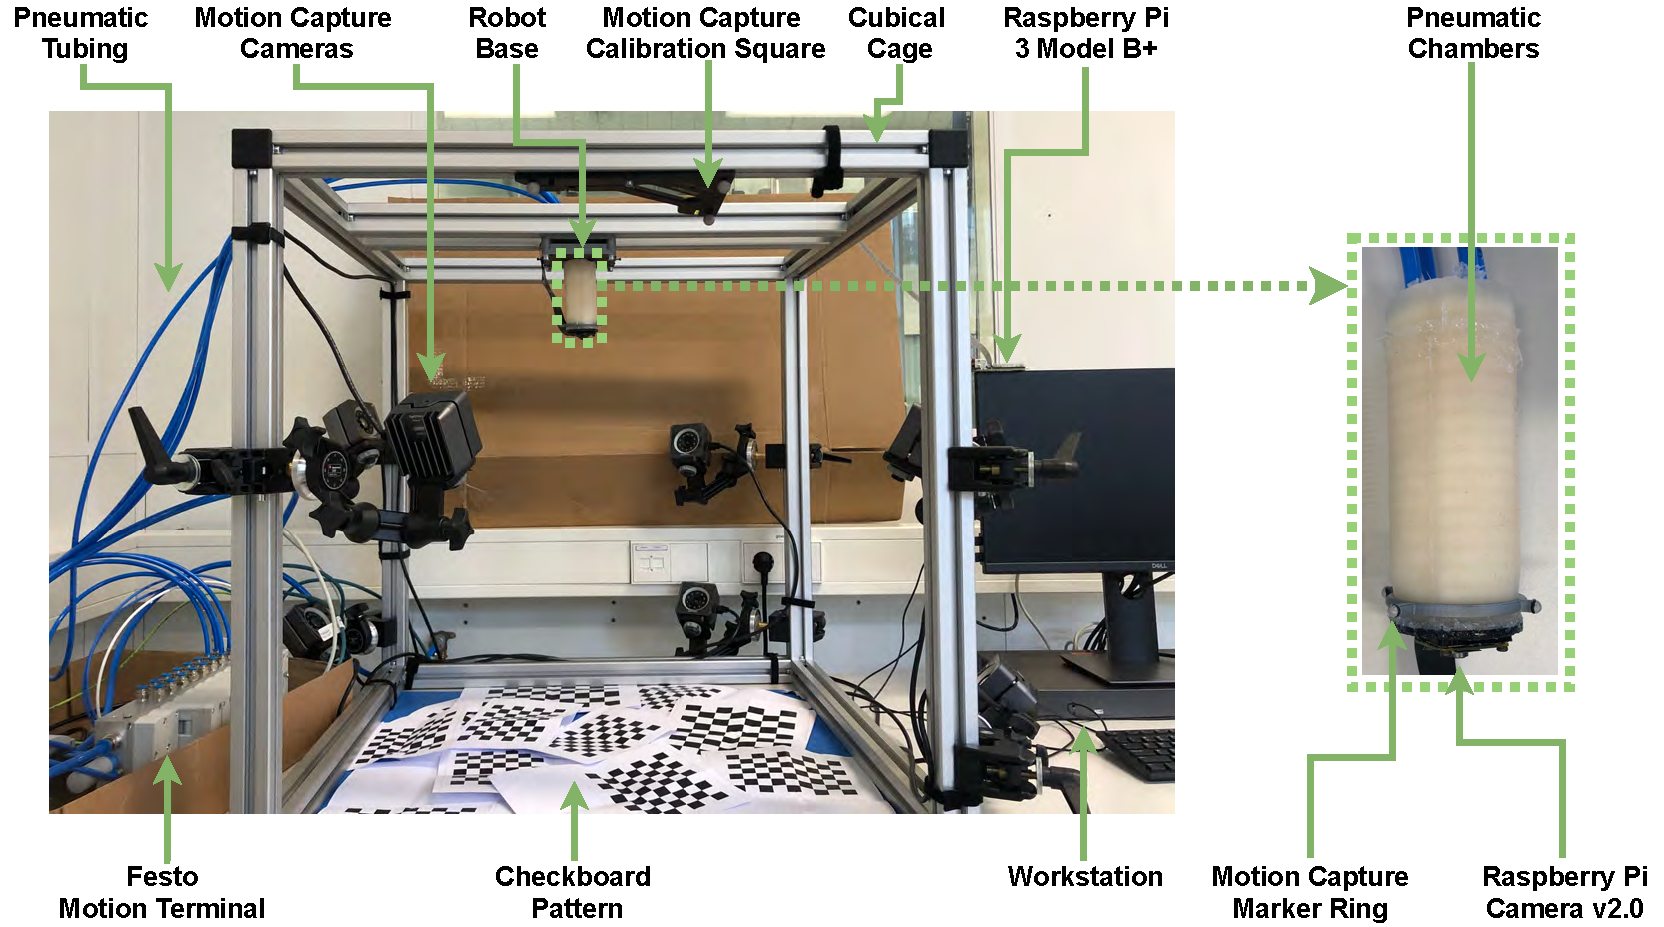
\includegraphics[height=.525\columnwidth]{srslam/figures/graphic_experimental_setup.drawio_v1_compressed.pdf} \label{fig:srslam:experimental_setup}}
     \subfigure[Trajectory 3]{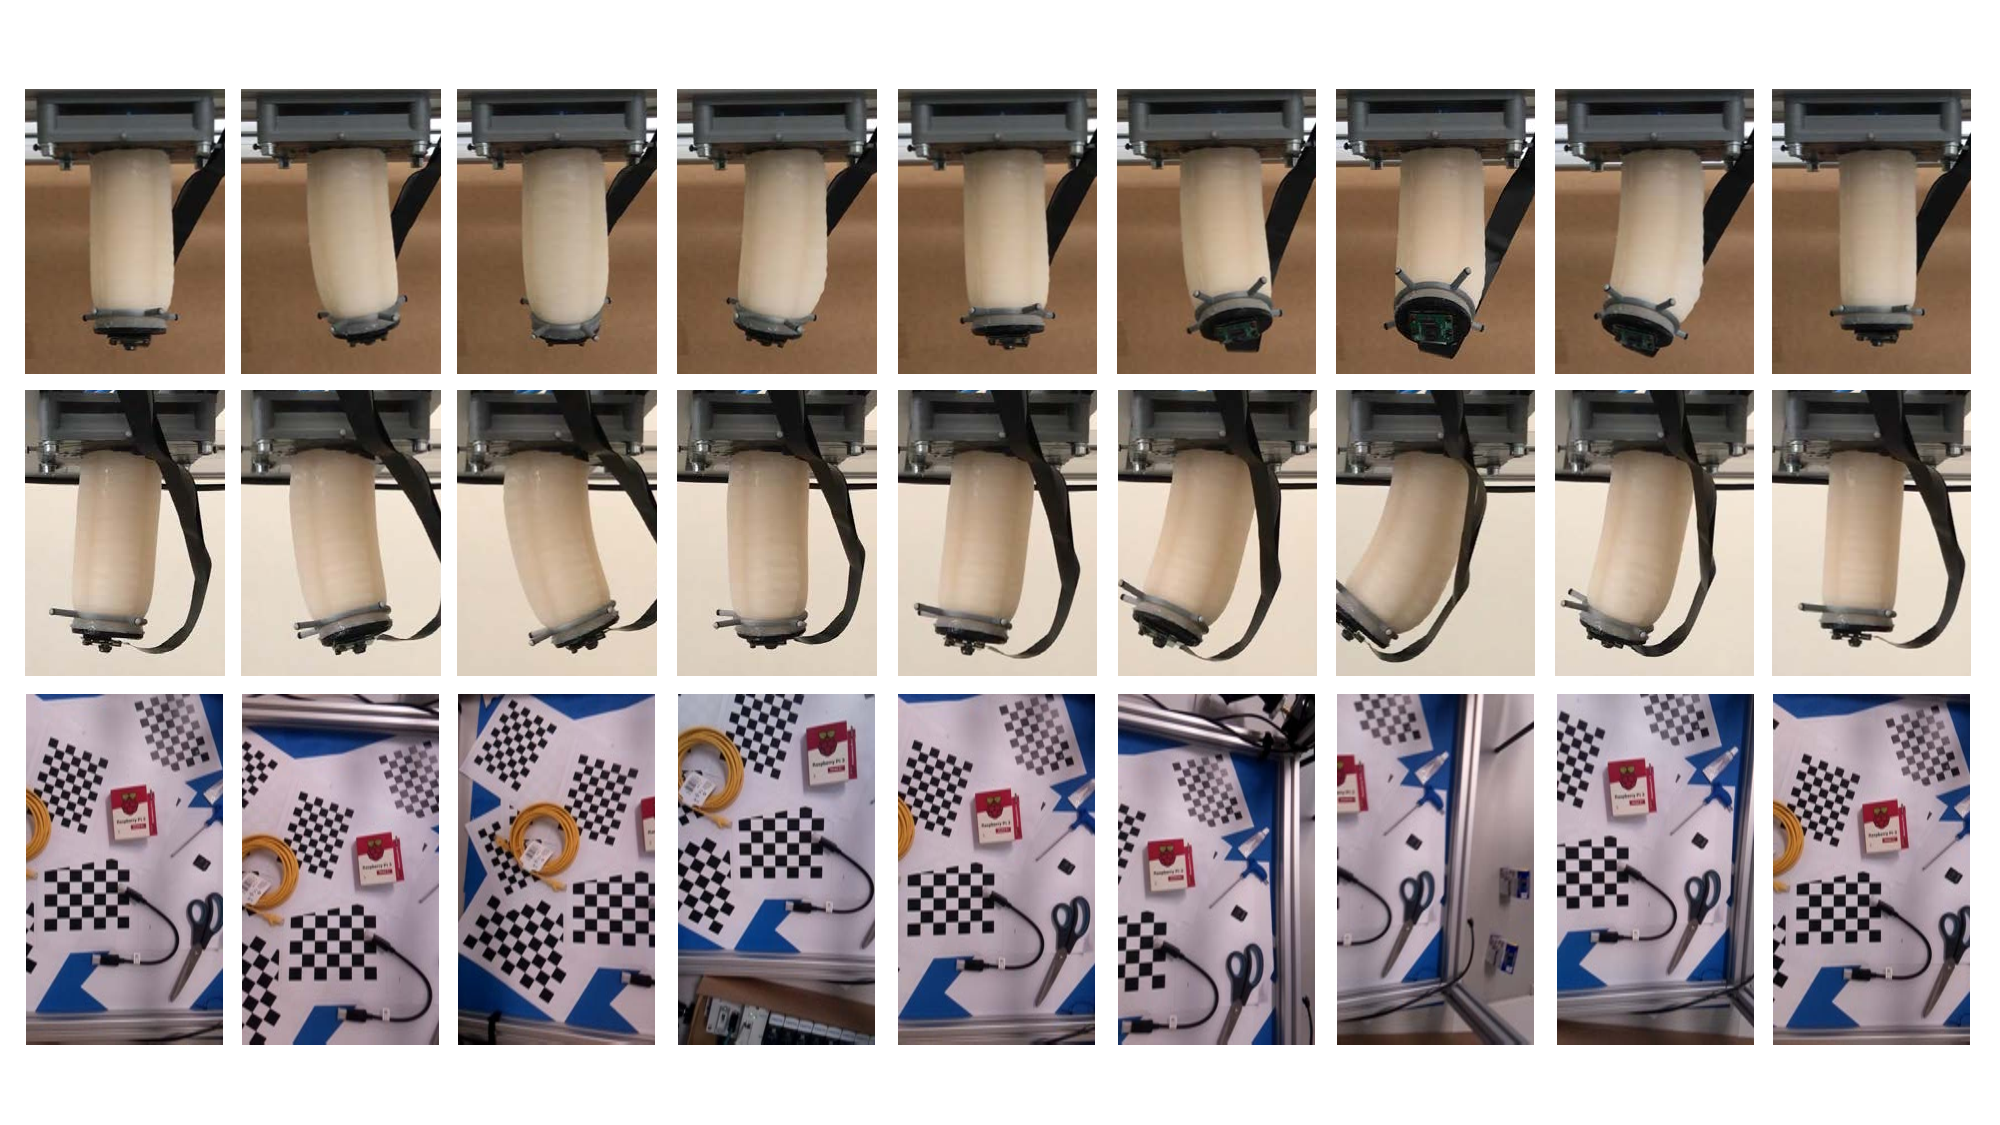
\includegraphics[height=.525\columnwidth]{srslam/figures/graphic_sequences_of_stills_lab_experiment_trajectory_3_compressed.pdf} \label{fig:srslam:graphic_sequences_of_stills_lab_experiment_trajectory_3}}
     \caption{ In Panel (a), a soft robotic segment is mounted to a cage with attached motion capture cameras. The segment is pneumatically actuated by a pressure regulator (Festo Motion Terminal). A Raspberry Pi camera v2.0 is attached to the tip of the segment and, in a straight segment configuration, looks down towards check-board patterns. Panel (b) depicts a sequence of stills showing the robot following trajectory 3 from two different vantage points. The second vantage point differs \SI{90}{\degree} from the first one. The third row displays a few representative frames, as recorded by the camera attached to the tip of the segment.}
\end{figure*}

\subsection{Experimental Setup}
% Segment and manufacturing
We show the experimental setup in Figure~\ref{fig:srslam:experimental_setup}.
We consider a soft robotic silicone segment consisting of four independently inflatable cavities. The segment has a cylindrical shape with a length $L_{0,1}$ of \SI{11}{cm} and a radius $d_1$ of \SI{21}{mm}. 
% We follow the fabrication procedure by \citet{marchese2015recipe} by casting Silicone into 3D-printed molds and block any silicon-flow into the air chambers with bees wax.
A 3D-printed ring with four motion capture markers is located near the tip of the segment.
%
% Camera and its attachment to the segment
We mount a Raspberry Pi camera module v2.0 to the tip of the segment.
This camera has a \SI{8}{MP} sensor and records frames at a sampling rate of \SI{30}{Hz} and a resolution of 1080p.
The focal length is \SI{3.04}{mm} and the field of view is $\SI{62.2}{\degree} \times \SI{48.8}{\degree}$.
The camera module is attached to a Raspberry Pi 3B+ single-board computer, which saves the frames for later processing by the ORB-SLAM~\citep{mur2017orb} algorithm.
The camera is screwed onto a custom 3D-printed holder, which in turn is glued with the tip plane of the segment.
%
% Actuation motion terminal, communication, commanding of pressures
The segment with its four air chambers is actuated with a proportional pressure regulator.
Tubing attached to the base of the segment connects each chamber with the assigned pneumatic valve of the pressure regulator.
%
% We apply a constant offset pressure $p_0$ to all chambers in straight configuration and subsequently synchronously increase the pressure $p_1$ in one chamber by $f_{\mathrm{p},x}$ and decrease the pressure in the opposite chamber $p_2$ by $f_{\mathrm{p},x}$ accordingly to cause a bending of the segment, in this case in x-direction.
% \begin{equation}
% \begin{split}
%     p_1 = p_0 - f_{\mathrm{p},x} \qquad p_2 = p_0 + f_{\mathrm{p},x}\\
%     p_3 = p_0 - f_{\mathrm{p},y} \qquad p_4 = p_0 + f_{\mathrm{p},y}
% \end{split}
% \end{equation}
% We map the desired configuration $\Delta_{x,1}$ and $\Delta_{y,1}$ given by the trajectories defined in \eqref{eq:srslam:trajectory_parametrization} in linear approximation to the commanded pressures
% \begin{equation}
%     f_{\mathrm{p},x} = a_x \; \Delta_{x,1} 
%     \qquad
%     f_{\mathrm{p},y} = a_y \; \Delta_{y,1}
%     \qquad
%     p_0 = a_{\delta L} \; \delta L_1
% \end{equation}
% where the proportional factors $a_{x}$, $a_{y}$ and $a_{\delta L}$ are experimentally determined and an elongation of the segment is reached through an increase in the offset pressure $p_0$.
% The pressure in each chamber is regulated by a Festo Motion Terminal using a factory-tuned PID controller.
% The commanded valve pressures are relayed via Modbus / TCP from our lab workstation to the Motion Terminal at a frequency of approximately \SI{10}{Hz}.
%
% Cage and environment
The segment is attached in an up-side-down configuration to the top plane of a cubical cage of \SI{750}{mm} side length. For a straight segment, the camera is facing downwards towards the floor of the cage, which is covered by multiple printed checkerboard patterns.
%
% Motion capture system and cage
We acquire ground-truth pose information of the tip of the segment using an Optitrack motion capture system. %, consisting of eight PrimeX 13 cameras mounted to the previously mentioned cubic cage. 
The ground-truth poses of the tip of the segment are recorded at \SI{30}{Hz}. % analogous to the Raspberry Pi camera frames.
% Additionally, we also record the pose of the base of the segment allowing us to determine a ground-truth coordinate transformation $T_{0}^{1}$ from the base to the tip.
%
% Implementation of PCC projection and calibration sequence
%In contrast to the model we used in simulation, the real-world segment experiences an elongation caused by the application of pressure to the chambers. Accordingly, 
%
We also include the elongation of the segment $\delta L_1$ in the cost function \eqref{eq:srslam:cost_fun} of our optimization.
%
% Calibration sequence
To resemble the calibration sequence from the simulation for the \gls{SLAM} map, we manually move the robot laterally into the x-coordinate direction before fixing it to the cage for the start of the experiments.

\subsection{Results}
Our experimental results reported in Table~\ref{tab:srslam:results_lab_experiments} and visualized for trajectory 3 in Figure~\ref{fig:srslam:experiments_t3_over_time} show translational relative \gls{RMSE} of between \SI{9}{\percent} and \SI{20}{\percent} for the three trajectories before optimization. 
The orientation of the z-axis of the tip is estimated with a mean error of approximately \SI{0.075}{\radian}.
The translational error is improved to between \SI{5}{\percent} and \SI{9}{\percent} after projection into the \gls{PCC}-kinematics. 
The optimization also slightly improves the rotational \gls{RMSE} by \SI{4}{\percent} to \SI{10}{\percent} relative to naive \gls{SLAM}.

The experimental results of the \gls{SLAM} algorithm are coherent with the simulations, as the small segment length (\SI{11}{cm}) used in the experiments increases the translational errors, as shown similarly in the simulations for a robot of length \SI{15}{cm}.
Even though the translational error is greatly reduced through optimization, it is still significantly higher than in simulation. Two reasons for this difference could be that a) the segment in the simulation was modeled as in-extensible, while the real robot segment is extended via pneumatic pressurization, which introduces additional errors by \gls{SLAM} not accurately estimating the elongation movement and b) the real robot does not perfectly behave according to the \gls{CC} approximation as the simulated robot does.

% \begin{table}
% \centering
% \caption{ \textcolor{orange}{OLD RESULTS: }oReal-world results before and after optimization: the translational errors are stated through a relative \gls{RMSE} and the rotational errors with an absolute \gls{RMSE} taking into account the Frobenius norm of the rotation matrices.}
% \begin{tabular}{lclll}\toprule
% \textbf{Error category} & \textbf{Opt.} & \textbf{Traj. 1} & \textbf{Traj. 2} & \textbf{Traj. 3}\\
% \midrule
% Translation $e_\mathrm{t}$ Eq.~\eqref{eq:srslam:evaluation_translational_error} & No & $\SI{24.8}{\percent}$ & $\SI{21.4}{\percent}$ & $\SI{9.5}{\percent}$ \\
% Translation $e_\mathrm{t}$ Eq.~\eqref{eq:srslam:evaluation_translational_error} & Yes & $\SI{11.4}{\percent}$ & $\SI{13.0}{\percent}$ & $\SI{4.5}{\percent}$ \\
% \midrule
% Rotation $e_\mathrm{R}$ Eq.~\eqref{eq:srslam:evaluation_rotational_error} & No & $0.105$ & $0.131$ & $0.116$ \\
% Rotation $e_\mathrm{R}$ Eq.~\eqref{eq:srslam:evaluation_rotational_error} & Yes & $0.098$ & $0.125$ & $0.112$ \\
% \midrule
% \textcolor{orange}{Rotation $e_{\theta_z}$ Eq.~\eqref{eq:srslam:evaluation_angle_error}} & No & $0.105$ & $0.131$ & $0.116$ \\
% \textcolor{orange}{Rotation $e_{\theta_z}$ Eq.~\eqref{eq:srslam:evaluation_angle_error}} & Yes & $0.098$ & $0.125$ & $0.112$ \\
% \bottomrule
% \end{tabular}
% \label{tab:srslam:results_lab_experiments}
% \end{table}

\begin{table}
\centering
\caption{ Real-world results before and after optimization. The translational errors are stated through a relative \gls{RMSE} as described in \eqref{eq:srslam:evaluation_translational_error}. For rotation, we report both an absolute \gls{RMSE} computed with the Frobenius norm between the rotation matrices as stated in \eqref{eq:srslam:evaluation_rotational_error} and an angle error [rad] for the orientation of the z-axis of the tip of the segment as defined in \eqref{eq:srslam:evaluation_angle_error}. The results are averaged over two trials for each trajectory.}
\begin{tabular}{lclll}\toprule
\textbf{Error category} & \textbf{Opt.} & \textbf{Traj. 1} & \textbf{Traj. 2} & \textbf{Traj. 3}\\
\midrule
Translation $e_\mathrm{t}$ & No & $\SI{20.3}{\percent}$ & $\SI{14.2}{\percent}$ & $\SI{9.1}{\percent}$ \\
Translation $e_\mathrm{t}$ & Yes & $\SI{9.1}{\percent}$ & $\SI{8.9}{\percent}$ & $\SI{5.0}{\percent}$ \\
\midrule
Rotation $e_\mathrm{R}$ & No & $0.145$ & $0.103$ & $0.126$ \\
Rotation $e_\mathrm{R}$ & Yes & $0.130$ & $0.099$ & $0.120$ \\
\midrule
Rotation $e_{\theta_z}$ & No & $\SI{0.079}{\radian}$ & $\SI{0.068}{\radian}$ & $\SI{0.084}{\radian}$ \\
Rotation $e_{\theta_z}$ & Yes & $\SI{0.080}{\radian}$ & $\SI{0.067}{\radian}$ & $\SI{0.084}{\radian}$ \\
\bottomrule
\end{tabular}
\label{tab:srslam:results_lab_experiments}
\end{table}

\begin{figure}[ht]
    \centering
    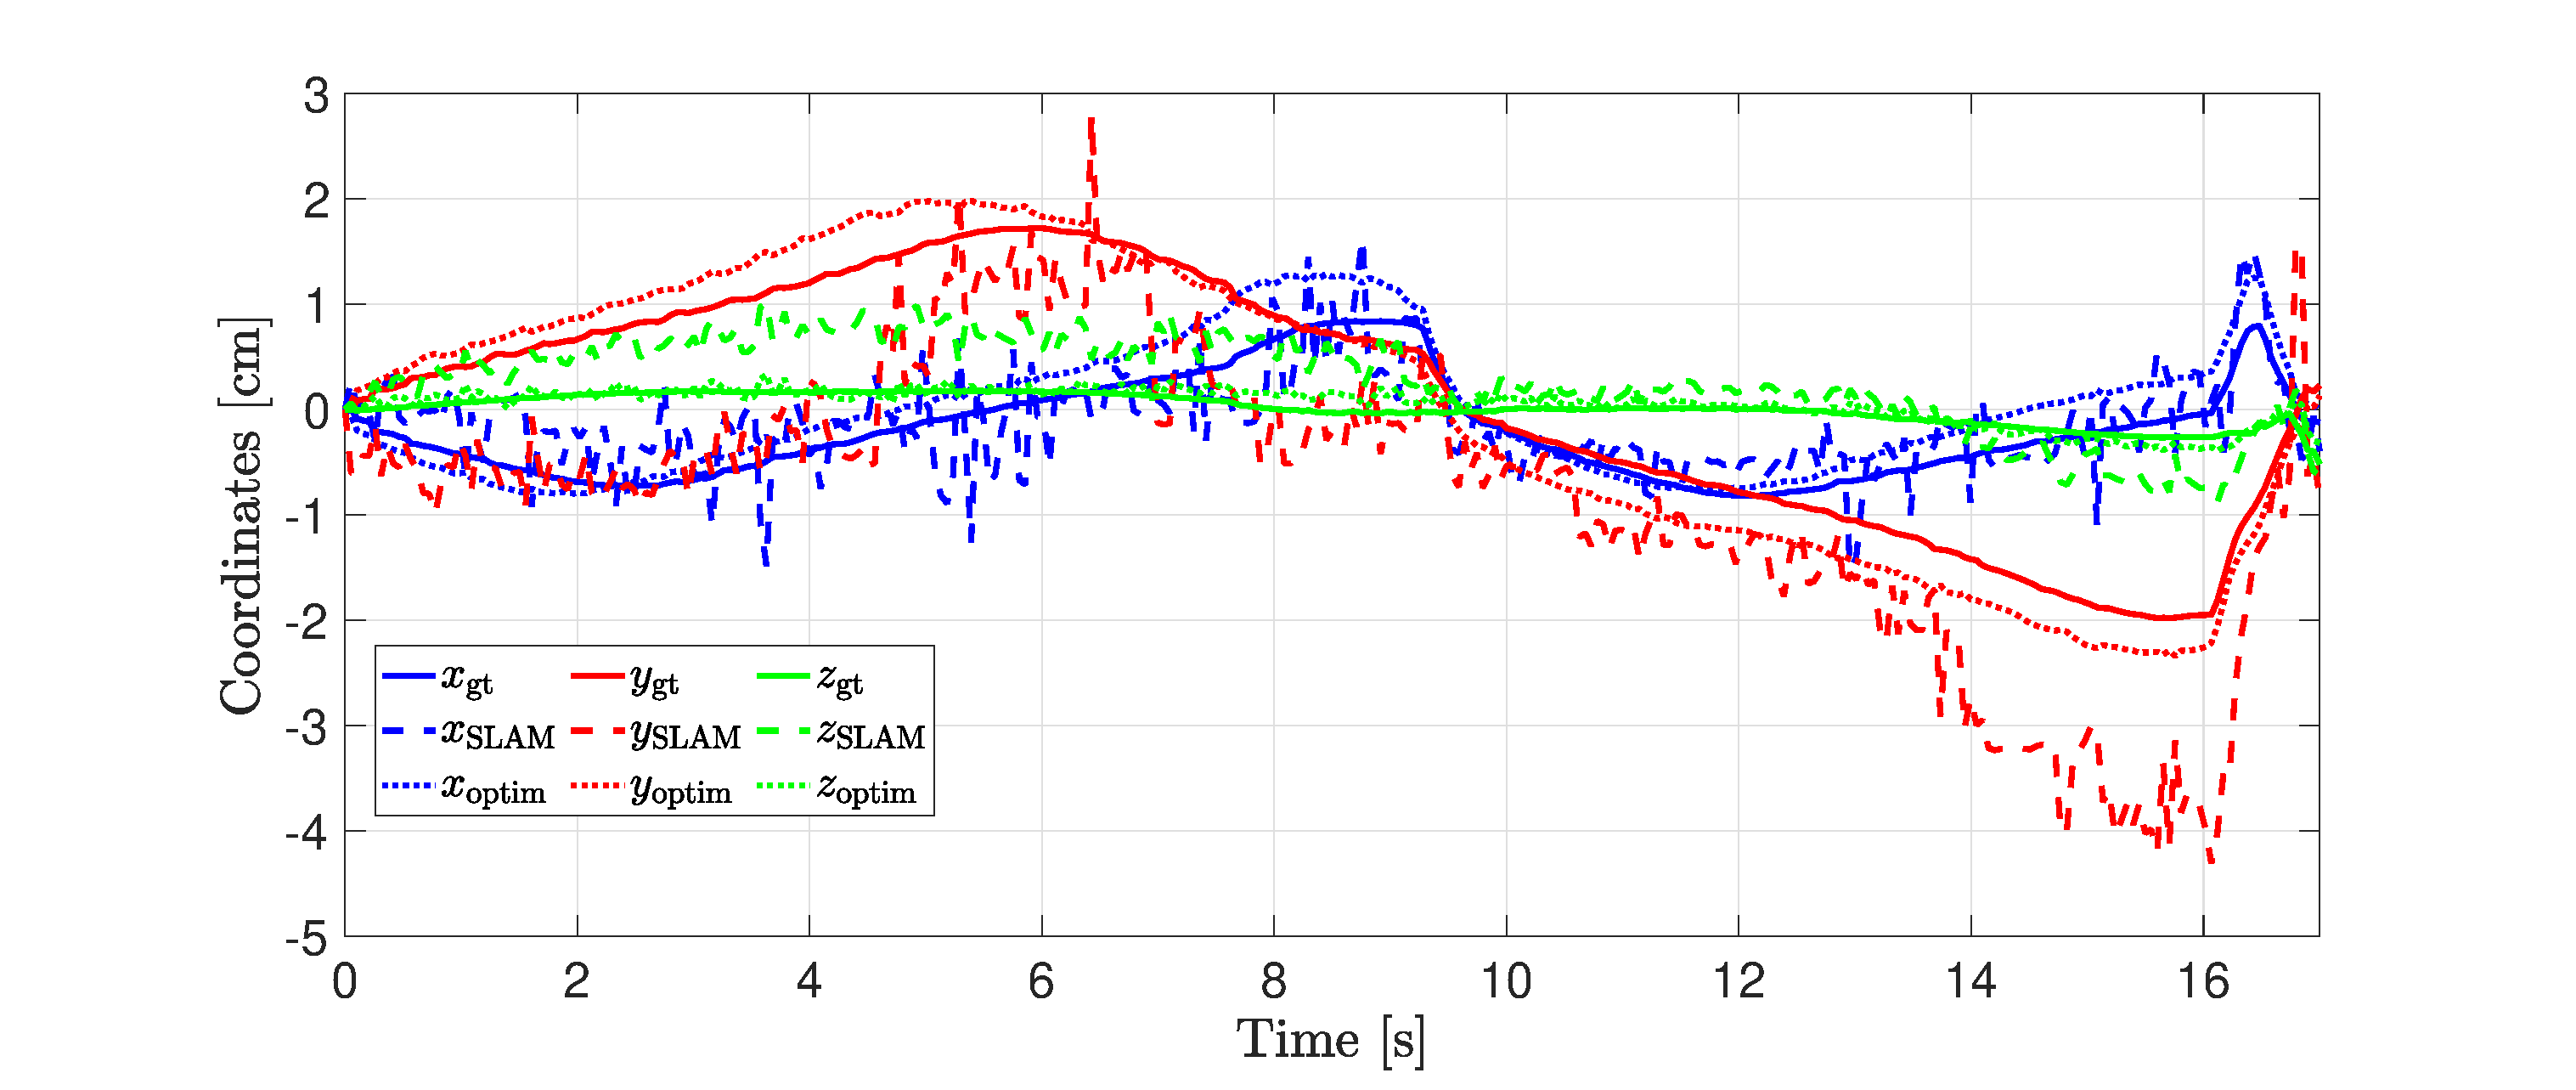
\includegraphics[width=0.9\columnwidth, trim={2cm 1.2cm 2cm 0}]{srslam/figures/vtem28_t3_coordinates.eps}\\
    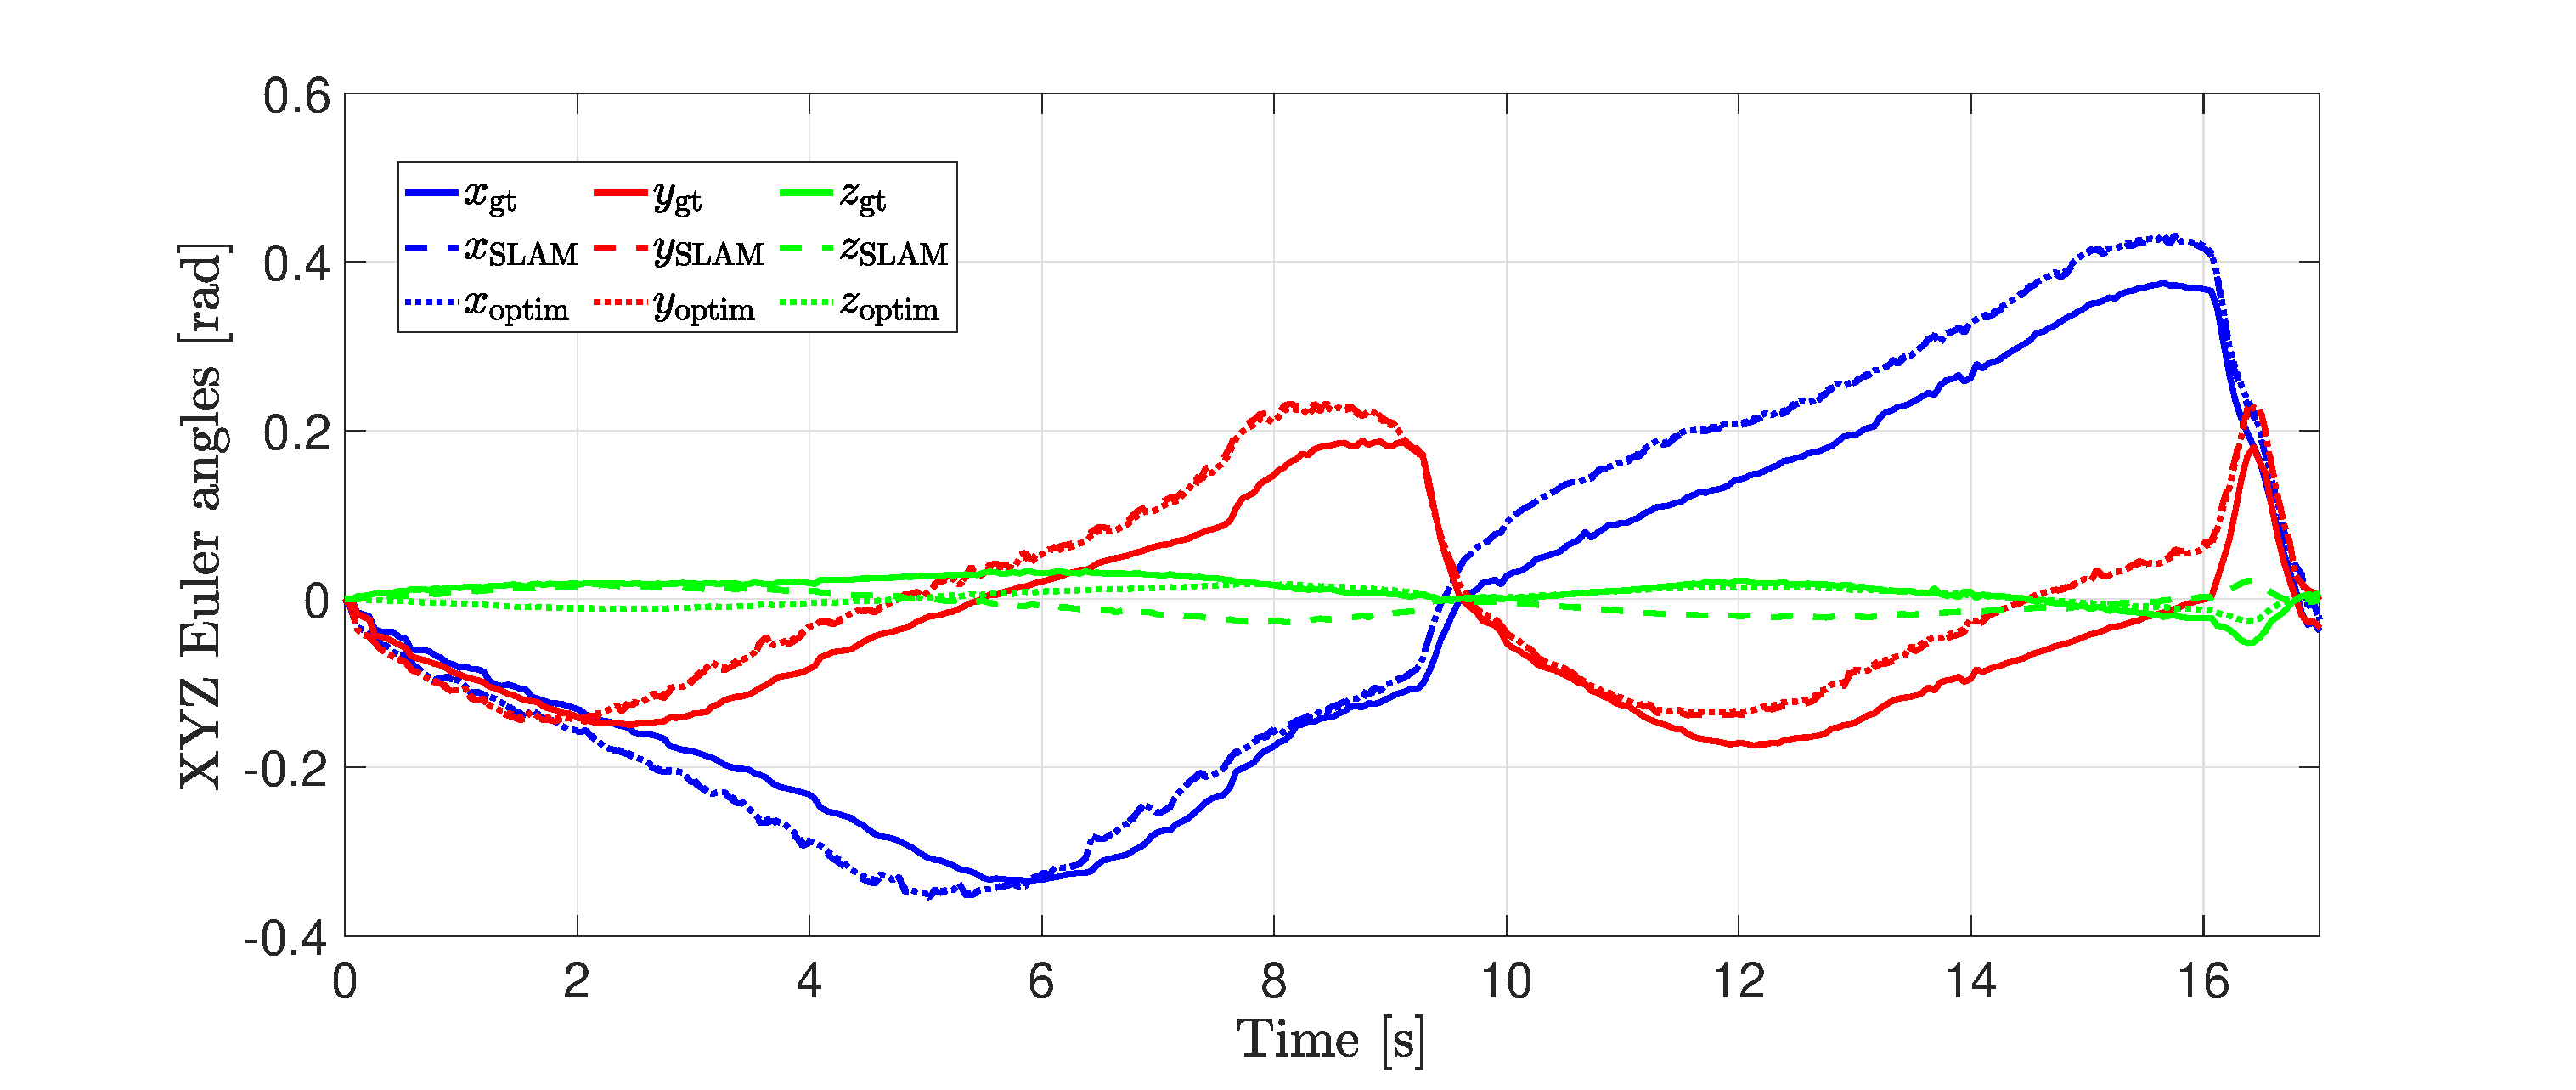
\includegraphics[width=0.9\columnwidth, trim={2cm 0 2cm 1.2cm}]{srslam/figures/vtem28_t3_angles.eps}
    \caption{ Experimental results for trajectory 3. Comparison between ground-truth (solid line), \gls{SLAM} (dashed line), and optimized through projection into \gls{PCC} kinematics (dotted line) for translation and orientation estimates.}
    \label{fig:srslam:experiments_t3_over_time}
\end{figure}


\section{Conclusion}
\label{sec:srslam:conclusions}

This paper investigated using a monocular camera in shape sensing of continuum soft robots, with the ultimate goal of implementing precise and reliable estimations at the cost of introducing small rigid parts into the hardware design. The contribution of this paper has been twofold. First, we proposed to use monocular SLAM with a soft robot. Second, we propose a regularization of the estimation based on a nonlinear projection in the manifold of admitted configuration. A nonlinear optimization implements the latter based on the kinematic model of the robot. We have performed extensive simulations with rendered images in Blender and lab experiments with a single segment soft robot. The nonlinear optimization based on the robot's kinematic model led to a significant improvement in translations and a marginal improvement in rotations. 
Future work will focus on extending the experimental validation of the method to multiple segments and cameras, bettering the SLAM by feeding back the kinematic projection in its state and using this estimation to implement closed-loop control.
While we conducted our experiments in a lab environment under ideal conditions with the camera pointed at checkerboard patterns thus resulting in plenty of image features for \gls{SLAM} to track, future work should investigate whether deployment environments for soft robots would be sufficiently feature-rich for the use of our proposed method.
